\documentclass[a4paper, 12pt]{article} % A4-Seitenformat und Schriftgröße 12pt

% Pakete für Sprache, Schrift und andere wichtige Anpassungen
\usepackage[utf8]{inputenc} % UTF-8 Unterstützung für Umlaute (ä, ü, ö)
\usepackage[T1]{fontenc}    % Korrekte Silbentrennung bei Umlauten
\usepackage[ngerman]{babel} % Deutsche Spracheinstellungen (z. B. Texttrennung, Typografie)
\usepackage{csquotes}       % Korrekte deutsche Anführungszeichen („ “)
\usepackage{hyperref} 		  % Klickbare Links im PDF
\usepackage{geometry}       % Seitenränder anpassen
\usepackage{float}					% Positionierung von Bildern und Tabellen

\usepackage{listings}			  % Code-Listings

\usepackage{tikz}           % Grafiken und Diagramme
% \tikzexternalize 					% Externe Speicherung von TikZ-Grafiken (schnelleres Kompilieren)
\usetikzlibrary{shadings}
\usetikzlibrary{calc,arrows.meta}

\usepackage{pgfplots}			  % Diagramme und Plots
\usepgfplotslibrary{external} % Externe Speicherung von Plots (schnelleres Kompilieren)
\pgfplotsset{compat=1.18}

\usepackage{fullpage} 		 	% Seitenränder auf 1 Zoll setzen
\usepackage{ulem} 				 	% Unterstreichungen und Durchstreichungen

\usepackage{amssymb,amsmath,changepage,tabularx,siunitx} % Mathematische Symbole und Umgebungen
\usepackage{darkmode}
\enabledarkmode 						% Dunkler Modus für bessere Lesbarkeit
\usepackage{makecell} 			% Tabellenzellen formatieren

\usepackage[most]{tcolorbox}
\definecolor{red1}{HTML}{ffccd5}
\definecolor{red2}{HTML}{ffb3c1}
\definecolor{red3}{HTML}{ff8fa3}
\definecolor{red4}{HTML}{ff758f}
\definecolor{red5}{HTML}{ff4d6d}
\definecolor{red6}{HTML}{c9184a}
\definecolor{red7}{HTML}{a4133c}
\definecolor{red8}{HTML}{800f2f}
\definecolor{red9}{HTML}{590d22} 
\definecolor{red10}{HTML}{c9181e}
\definecolor{red11}{HTML}{c91876}
\definecolor{red12}{HTML}{e5235a}
\definecolor{pag}{HTML}{293133}
	\usepgfplotslibrary{colormaps,patchplots}
\definecolor{cbada55}{RGB}{186,218,85}
\definecolor{c2c2c2c}{RGB}{44,44,44}
\definecolor{cc9184a}{RGB}{201,24,74}
\definecolor{c8d354e}{RGB}{141,53,78}
\definecolor{cff4d6d}{RGB}{255,77,109}
\definecolor{cff758f}{RGB}{255,117,143}
		\usetikzlibrary{3d,perspective}

\newtcolorbox{qq}[2][]{  
	boxrule=0.75pt, % Thin border
	sharp corners, 	% Square edges
	colframe=white, % Set the color of the outline
	colback=pag,  	% Set the color of the fill
	coltext=white,	% Set the color of the text
	#1,							% Other options
}

\lstset{
  basicstyle=\ttfamily,
  keywordstyle=\bfseries\color{red3},
  commentstyle=\itshape\color{red12},
  stringstyle=\color{red5},
  numbers=left,
  numberstyle=\small,
  stepnumber=1,
  breaklines=true,
	frame=single,
	backgroundcolor=\color{pag},
	captionpos=b,
	xleftmargin=0.1cm,
	xrightmargin=0.1cm,	
}

% JavaScript definieren
\lstdefinelanguage{JavaScript}{
    keywords={break,case,catch,class,const,continue,debugger,default,delete,do,
      else,export,extends,finally,for,function,if,import,in,instanceof,let,new,
      return,super,switch,this,throw,try,typeof,var,void,while,with,yield, from},
    sensitive=true,
    morecomment=[l]{//},
    morecomment=[s]{/*}{*/},
    morestring=[b]",
    morestring=[b]'
}

% Python definieren
\lstdefinelanguage{Python}{
	keywords={},
	sensitive=true,
	morecomment=[l]{\#},
	morestring=[b]',
	morestring=[b]",
}

\usepackage{mathpazo} % Palatino Schriftart

\usetikzlibrary{decorations.markings,arrows.meta,bending}
\usepackage{tikz-3dplot}
\usetikzlibrary{3d,backgrounds,intersections}

\makeatletter
\tikzoption{canvas is xy plane at z}[]{%
	\def\tikz@plane@origin{\pgfpointxyz{0}{0}{#1}}%
	\def\tikz@plane@x{\pgfpointxyz{1}{0}{#1}}%
	\def\tikz@plane@y{\pgfpointxyz{0}{1}{#1}}%
	\tikz@canvas@is@plane}
\makeatother

\usepgfplotslibrary{groupplots}
\usepgfplotslibrary{fillbetween}

\usepackage{colortbl}
\usepackage{caption}
\usepackage{polynom}
\usepackage[backend=biber]{biblatex}

% \usepackage[top=1in,bottom=1in,right=1in,left=1in]{geometry}
% \usepackage{mdframed}
\usepackage{array}
\usepackage{multirow}
\definecolor{pagtwo}{HTML}{3E4547}

\geometry{a4paper, left=3cm, right=3cm, top=2.5cm, bottom=2.5cm} % Beispiel für Seitenränder

\title{Automatisierter Smarter Cocktail-Automat mit Cloud Anbindung}
\author{ 
  Jonas Eck \\
	Technische Hochschule Würzburg-Schweinfurt\\
	\and 
	Phillip Schön \\
	Technische Hochschule Würzburg-Schweinfurt\\
	\and 
  Constantin Thein\\
	Technische Hochschule Würzburg-Schweinfurt\\
	}

\date{\today}

% TODO: 
% - [x] Einleitung
% - [x] Technologischer Hintergrund und Grundlagen
% - [x] Anforderungen und Konzept
% - [ ] Umsetzung der Hardware
% - [x] Backend-Architektur und Implementierung
% - [ ] Mobile App-Entwicklung
% - [ ] Integration und Tests 
% - [ ] Ergebnisse und Bewertung 
% - [ ] Fazit und Ausblick 
% - [ ] Anhang
% - [ ] Literaturverzeichnis
% - [ ] Interaktionen zwischen Komponenten - Abbildung, in 3.5

\linespread{1.5}

\addbibresource{literaturverzeichnis.bib}

\begin{document}

\maketitle
\newpage
\tableofcontents
\newpage

\begin{abstract}
Im Rahmen dieses Projekts wurde ein smarter Cocktailautomat entwickelt, der wesentliche Elemente des
Internet of Things (IoT) mit den Anforderungen moderner Smart-Home-Lösungen verbindet. Ziel war die
Umsetzung eines skalierbaren Prototyps, der die automatisierte Zubereitung von Cocktails ermöglicht 
und dabei durch eine intuitive Bedienung über eine Smartphone-App sowie die Anbindung an ein 
cloudbasiertes Backend besticht.

Die Lösung umfasst drei Kernkomponenten: eine modular aufgebaute Hardware für die 
Cocktailzubereitung, ein containerisiertes Backend gehostet in Google Cloud Run mit einer 
Cloud-SQL-Datenbank sowie eine mobile App, die eine benutzerfreundliche Verwaltung von Rezepten, 
Zutaten und Maschinenkonfigurationen erlaubt. Besonderes Augenmerk wurde auf die Skalierbarkeit und 
Erweiterbarkeit des Systems gelegt, wodurch sowohl mehrere Benutzer als auch mehrere Automaten 
unterstützt werden können.

Das Projekt zeigt die Potenziale von IoT-Technologien auf, alltägliche Aufgaben zu automatisieren 
und dabei innovative Ansätze für Smart-Home-Umgebungen zu entwickeln. Gleichzeitig wurden 
Herausforderungen wie die Einarbeitung in neue Technologien, der Umgang mit komplexen 
Elektronikkomponenten sowie die effiziente Integration von Cloud-Diensten gemeistert.
\end{abstract}
\newpage

\section{Einleitung}
\subsection{Motivation}
Die Idee eines smarten Cocktailautomaten entstand im Kontext unserer Erfahrungen beim Organisieren 
und Betreiben von Cocktailbars auf Fakultätsveranstaltungen. Diese praktischen Erfahrungen zeigten, 
wie zeitaufwendig die manuelle Zubereitung von Cocktails insbesondere bei hohem Gästeaufkommen sein 
kann. Mit der zunehmenden Verbreitung von Smart-Home-Geräten und IoT - Lösungen kam die Idee auf, 
diesen Prozess durch Automatisierung zu vereinfachen und so die Cocktailzubereitung effizienter und 
benutzerfreundlicher zu gestalten. 
\\
Ein weiterer Beweggrund war die Möglichkeit, aktuelle Technologien wie Cloud-Computing und mobile 
Anwendungen in einer praxisnahen IoT - Anwendung zu integrieren und deren Potenzial in einem kreativen 
Projekt auszuloten. Während der COVID-19 - Pandemie entstanden zahlreiche Do-it-yourself-Projekte im 
Bereich der Automatisierung, welche uns zu dieser Idee inspirierten.

\subsection{Zielsetzung}
Das Hauptziel des Projekts war die Entwicklung eines skalierbaren Prototyps, der die 
Cocktailzubereitung durch Automatisierung weitgehend vereinfacht. Die Bedienung des Automaten 
sollte intuitiv und nutzerfreundlich sein, sodass Benutzer per Smartphone-App mit wenigen Klicks 
einen Cocktail 'auf Knopfdruck' zubereiten können. Um eine hohe Flexibilität und Erweiterbarkeit 
zu gewährleisten, wurde eine Cloud - basierte Architektur gewählt, die es ermöglicht, mehrere 
Automaten gleichzeitig zu steuern oder eine Maschine mehreren Benutzern zugänglich zu machen. 

Ein weiterer Aspekt des Projekts war der Fokus auf Kosteneffizienz: Ziel war es, eine Lösung zu 
entwickeln, die im Vergleich zu bestehenden kommerziellen Produkten kostengünstiger ist, ohne dabei 
an Funktionalität und Skalierbarkeit einzubüßen.

\subsection{Relevanz}
Das Projekt verbindet aktuelle Trends im Bereich der Smart-Home-Technologien mit praxisorientierten 
Anwendungen des Internet of Things (IoT). Insbesondere die Integration von Cloud-Diensten und 
mobilen Applikationen in eine physische Maschine bietet ein breites Anwendungsfeld für ähnliche 
Automatisierungslösungen, die über den Cocktailautomaten hinausgehen. Durch den Prototyp wird 
gezeigt, wie IoT-Technologien genutzt werden können, um alltägliche Prozesse effizienter zu 
gestalten. 

Darüber hinaus stellt das Projekt eine wertvolle Gelegenheit dar, sich mit modernen Cloud-
Technologien wie Google Cloud Run und Cloud SQL sowie mit der Entwicklung mobiler Anwendungen und 
hardwarebezogener Softwarelösungen auseinanderzusetzen. Dies spiegelt die zunehmende Relevanz 
solcher Technologien in der Industrie wider.

\subsection{Überblick über die Arbeit}
Die vorliegende Projektarbeit gliedert sich wie folgt: Zunächst wird der technologische Hintergrund 
des Projekts vorgestellt, inklusive einer Einführung in IoT und Smart-Home-Systeme sowie der 
verwendeten Technologien. Anschließend werden die Anforderungen und das Konzept des Cocktail-
Automaten dargelegt. Die darauf folgenden Kapitel widmen sich der Umsetzung der drei zentralen 
Komponenten des Systems: der Hardware, dem containerisierten Backend sowie der mobilen App. 

Im weiteren Verlauf wird die Integration der Komponenten beschrieben und die durchgeführten Tests 
dokumentiert. Abschließend werden die erzielten Ergebnisse zusammengefasst, eine kritische Bewertung
 vorgenommen und ein Ausblick auf mögliche Weiterentwicklungen gegeben. Herausforderungen wie der 
 Umgang mit neuen Technologien, die Skalierung des Systems sowie der zeitliche Umfang des Projekts 
 werden im Rahmen der Arbeit reflektiert.

    
\newpage

\section{Technologischer Hintergrund und Grundlagen}(3–5 Seiten)
\section{Technologischer Hintergrund und verwandte Arbeiten}
% Hier folgt der Inhalt des Abschnitts "Technologischer Hintergrund und verwandte Arbeiten".
    
\newpage

\section{Anforderungen und Konzept}(4–5 Seiten)
% Hier folgt der Inhalt des Abschnitts "Anforderungen und Konzept".
Im Rahmen des Projekts „Smarter Cocktailautomat“ wurden grundlegende Anforderungen definiert, die 
sich aus den Zielsetzungen und den zu erwartenden Einsatzszenarien ableiten lassen. Dieser 
Abschnitt gliedert sich in eine Analyse der funktionalen und nicht-funktionalen Anforderungen 
sowie die Entwicklung eines konzeptionellen Architekturansatzes, der die Interaktionen zwischen 
Hardware, Backend und mobiler App beschreibt.

\subsection{Anforderungsanalyse}

Die Anforderungsanalyse bildet die Grundlage für die Entwicklung des Prototyps. Dabei werden 
sowohl funktionale als auch nicht-funktionale Anforderungen betrachtet.

\subsection{Funktionale Anforderungen}

Funktionale Anforderungen beschreiben die Kernfunktionen, die das System erfüllen muss, um die 
Projektziele zu erreichen:

\begin{itemize}
	  \item \textbf{Benutzerregistrierung und -verwaltung:} Möglichkeit, Benutzerkonten anzulegen, zu bearbeiten und zu löschen.
	  \item \textbf{Rezeptverwaltung:} Hinzufügen, Bearbeiten und Löschen von Cocktailrezepten über die mobile App.
	  \item \textbf{Zutatenverwaltung:} Verwaltung der im Automaten verfügbaren Zutaten mit Anzeige von Füllständen.
	  \item \textbf{Automatisierte Zubereitung:} Präzise Dosierung und Mischung der ausgewählten Zutaten basierend auf den Rezepten.
	  \item \textbf{App-Steuerung:} Steuerung des Cocktailautomaten über eine intuitive Benutzeroberfläche der mobilen App.
	  \item \textbf{Synchronisation mit der Cloud:} Speicherung und Abruf von Benutzerdaten, Rezepten und Maschinenkonfigurationen über ein cloudbasiertes Backend.
\end{itemize}

\subsection{Nicht-funktionale Anforderungen}

Neben den funktionalen Aspekten spielen auch nicht-funktionale Anforderungen eine zentrale Rolle, 
um die Qualität und Benutzerfreundlichkeit des Systems sicherzustellen:

\begin{itemize}
	  \item	\textbf{Skalierbarkeit:} Das System muss in der Lage sein, mehrere Benutzer und Automaten zu unterstützen, ohne Leistungseinbußen zu erleiden.
	  \item	\textbf{Sicherheitsaspekte:} Schutz von Benutzerdaten durch verschlüsselte Kommunikation und sichere Authentifizierungsverfahren.
	  \item	\textbf{Benutzerfreundlichkeit:} Intuitive Bedienung der mobilen App sowie einfache Wartung und Erweiterung der Hardware.
	  \item	\textbf{Fehlerresistenz:} Robustheit des Systems gegenüber Hardware- und Softwarefehlern.
	  \item	\textbf{Performance:} Minimierung von Latenzen bei der Kommunikation zwischen App, Backend und Hardware.
\end{itemize}

\subsection{Konzeptionelle Architektur}

Auf Basis der definierten Anforderungen wurde eine konzeptionelle Architektur entwickelt, die das 
Gesamtsystem in seinen zentralen Komponenten beschreibt.

Gesamtsystem-Übersicht

Das System besteht aus drei Kernkomponenten:

\begin{enumerate}
  \item \textbf{Hardware:} Der Cocktailautomat als physisches Gerät übernimmt die Dosierung und Mischung der Zutaten.
  \item \textbf{Backend:} Ein containerisiertes Backend, das in Google Cloud Run gehostet wird, dient als zentrale Schnittstelle für die Speicherung und Verarbeitung von Daten.
  \item \textbf{Mobile App:} Eine Smartphone-App ermöglicht die Benutzerinteraktion mit dem System und bietet Funktionen wie Rezeptverwaltung und Steuerung des Automaten.
\end{enumerate}

Die Interaktionen zwischen diesen Komponenten sind in Abbildung \ref{fig:system_overview} 
dargestellt. Dabei wird insbesondere der Datenfluss zwischen den Modulen hervorgehoben.

\vspace{0.5 cm}
\begin{figure}[htbp]
  \centering
	\begin{tikzpicture}[
		>=stealth,   					% Standardpfeilspitzen
		outer sep=6pt,				% Abstand zwischen Text und Rahmen
		inner sep=5pt,				% Abstand zwischen Text und Rahmen
		node distance=6cm,	% Abstand zwischen den Knoten
		font=\sffamily				% Verwendete Schriftart
	]
	
	% Knoten
	\node[draw, rectangle, rounded corners, fill=red3, minimum width=2.5cm, minimum height=1.2cm] (hardware) {Hardware};
	\node[draw, rectangle, rounded corners, fill=red3, minimum width=2.5cm, minimum height=1.2cm, left of=hardware] (backend) {Backend};
	\node[draw, rectangle, rounded corners, fill=red3, minimum width=2.5cm, minimum height=1.2cm, left of=backend] (app) {Mobile App};
	
	% Pfeil 1: ein Wort pro Zeile, zentriert
	\draw[<-, thick] 
	(hardware) 
	-- node[below]{
		\parbox{2.7cm}{\centering
			Rezeptdaten,\\
			Slotbestückung 
		}
	} 
	(backend);

	% Pfeil 2: ein Wort pro Zeile, zentriert
	\draw[<->, thick] 
	(app) 
	-- node[below]{
		\parbox{2.7cm}{\centering
			Benutzerdaten,\\
			Rezepte \&\\
			Konfiguration
		}
	} 
	(backend);

	\end{tikzpicture}

	\caption{Systemübersicht: Interaktionen zwischen Hardware, Backend und mobiler App}
	\label{fig:system_overview}
\end{figure}

\paragraph*{Datenflüsse und Interaktionen}

\begin{itemize}
  \item Die Hardware kommuniziert mit dem Backend, um die aktuellen Maschinenzustände zu synchronisieren.
  \item Die mobile App greift auf das Backend zu, um Benutzerdaten, Rezepte und Maschinenkonfigurationen zu laden und zu speichern.
  \item Das Backend dient als zentrale Vermittlungsstelle und verarbeitet sowohl Steuerbefehle von der App als auch Statusmeldungen der Hardware.
\end{itemize}

\subsection{Schwerpunktsetzung}

Im Rahmen des Projekts wurde besonderes Augenmerk auf die folgenden Aspekte gelegt:

\begin{itemize}
  \item \textbf{Hardware:} Die Hardwareentwicklung zielte auf eine modulare und erweiterbare Bauweise ab, um zukünftige Anpassungen und Erweiterungen zu ermöglichen.
  \item \textbf{Backend:} Aufgrund der hohen Anforderungen an Skalierbarkeit und Sicherheit wurde das Backend so konzipiert, dass es sowohl eine zuverlässige Kommunikation zwischen den Komponenten als auch eine effiziente Datenverwaltung ermöglicht.
  \item \textbf{Mobile App:} Der Fokus lag auf einer benutzerfreundlichen und intuitiven Bedienung, um die Nutzung auch für technisch unerfahrene Anwender zu vereinfachen.
\end{itemize}
    
\newpage

\section{Umsetzung der Hardware}(4–6 Seiten)
\subsection{Überblick}
Die Hardwareplattform für das Projekt bildet das Herzstück des Cocktailautomaten und wurde mit dem Ziel ausgewählt, eine robuste und flexible Steuerung der mechanischen und elektronischen Komponenten zu gewährleisten. Die Wahl fiel auf den \textbf{Raspberry Pi Zero 2 W}, eine kompakte und leistungsfähige Single-Board-Computer-Lösung, die sich aufgrund ihrer Vielseitigkeit und der umfangreichen Unterstützung von Python-Bibliotheken ideal für IoT-Anwendungen eignet. Ergänzt wird der Raspberry Pi durch eine Vielzahl von Sensoren, Aktoren und Peripheriegeräten, die zusammen die präzise Steuerung des Automaten ermöglichen.

\subsection{Zentrale Steuerung}
Der Raspberry Pi Zero 2 W übernimmt die zentrale Steuerung des Systems. Mit einem Quad-Core ARM Cortex-A53-Prozessor und integrierter WLAN- und Bluetooth-Konnektivität eignet sich der Pi optimal für die Verarbeitung der Steuerungslogik und die Kommunikation mit dem Backend.

\subsection{Mechanische Komponenten}
\subsubsection{Schrittmotor für die Positionierung}
Ein Schrittmotor steuert die präzise Bewegung eines Förderbandsystems, welches die verschiedenen Getränkezutaten anfahren kann. Mit einem Dir- und Pul-Pin-Design wird der Schrittmotor über einen \textbf{Treiber} angesteuert, der eine feine Steuerung der Bewegung und Geschwindigkeit ermöglicht. Ein Schlitten bewegt sich zwischen den Slots, die durch Endschalter (Limit Switches) abgegrenzt sind.

\subsubsection{Linearantrieb für alkoholische Getränke}
Ein Linearmotor aktiviert die Dosiermechanismen für alkoholische Zutaten, die kopfüber montiert sind. Der Antrieb hebt die Dosiermechanik an, um Flüssigkeiten aus den Flaschen freizugeben, und stellt sicher, dass die gewünschte Menge präzise abgefüllt wird.

\subsubsection{Membranpumpen für nicht-alkoholische Zutaten}
Sechs Membranpumpen sind für die Abgabe von nicht-alkoholischen Zutaten zuständig. Diese Pumpen ermöglichen eine genaue Dosierung der Flüssigkeiten und werden einzeln über GPIO-Pins des Raspberry Pi angesteuert. Jede Pumpe ist einem festen Slot zugewiesen.

\subsection{Sensorik}
\subsubsection{Endschalter für die Positionserkennung}
Sechs Endschalter (Limit Switches) überwachen die genaue Position des Schlittenmechanismus. Endschalter 0 ist für die Kalibrierung vorgesehen und dient als Referenzpunkt. Außerdem werden an diesem Punkt die nicht-alkoholischen Getränke am Ende der Zubereitung zugefügt. Die übrigen Schalter (1--5) bilden die Position der Slots für alkoholische Getränke (ebenfalls 1--5) ab.

\subsubsection{Waage für Gewichtsmessung}
Eine elektronische Waage auf Basis eines HX711-Sensors misst das Gewicht der Getränke während der Zubereitung. Sie dient nicht nur der Überwachung der genauen Flüssigkeitsmengen, sondern auch der Erkennung, ob eine Zutat aufgebraucht ist.

\subsection{Stromversorgung}
Die gesamte Hardware wird von einem \textbf{24V-Netzteil} mit ausreichender Leistung (mindestens 3A) versorgt. Zwei \textbf{Step-Down-Spannungsregler} wandeln die Spannung auf 5V respektive 12V für den Raspberry Pi und weitere elektronische Komponenten um. Zur Vermeidung von Spannungsschwankungen und elektromagnetischen Störungen wurden \textbf{Kondensatoren} integriert, die die Stabilität der Stromversorgung sicherstellen.

\subsection{Zusammenarbeit der Komponenten}
Alle Hardwarekomponenten arbeiten nahtlos zusammen, um die Zubereitung eines Cocktails zu automatisieren:
\begin{itemize}
    \item Die \textbf{Positionserkennung} sorgt dafür, dass der Schlitten immer die korrekte Position ansteuert.
    \item Die \textbf{Waage} und die Pumpen oder der Linearantrieb arbeiten zusammen, um die exakte Menge jeder Zutat abzugeben.
\end{itemize}

\subsection{Integration und Herausforderungen}
Die Integration der verschiedenen Hardwarekomponenten erforderte eine sorgfältige Planung, insbesondere bei der Belegung der GPIO-Pins und der Kalibrierung der Sensoren. Eine besondere Herausforderung stellte die Stabilität der Stromversorgung dar, insbesondere bei Spitzenlasten durch den Schrittmotor oder die Pumpen. Durch die Verwendung eines ausreichend dimensionierten Netzteils und der Optimierung des Codes konnte dieses Problem erfolgreich gelöst werden.
    
\newpage

\section{Backend-Architektur und Implementierung}(4–6 Seiten)
% Hier folgt der Inhalt des Abschnitts "Backend-Architektur und Implementierung".
Das Backend bildet das zentrale Bindeglied zwischen der mobilen App, der Hardwarekomponente des 
Cocktailautomaten und der cloudbasierten Datenbank. Es ist dafür verantwortlich, Datenflüsse zu 
koordinieren, Benutzer- und Rezeptinformationen zu verwalten und eine nahtlose Kommunikation 
zwischen den Systemkomponenten zu gewährleisten.

\subsection{Allgemeine Architektur}

Das Backend folgt einer einfachen serverbasierten Struktur und stellt HTTP - Endpunkte bereit, die 
von der mobilen App aufgerufen werden können. Diese Endpunkte aktivieren spezifische Handler-
Funktionen, die in der Regel direkte Datenbankoperationen ausführen. Zusätzlich ermöglicht das 
Backend über eine Websocket-Schnittstelle die Kommunikation mit der Hardware, um Bestellungen in 
Echtzeit an die Geräte weiterzuleiten.

Technologisch basiert das Backend vollständig auf Golang, unterstützt durch Frameworks wie \texttt{
gorilla/ mux} für die Routenverwaltung und \texttt{database/sql} für den Zugriff auf die PostgreSQL 
- Datenbank. Die gesamte Umgebung ist containerisiert und nutzt Docker Compose für lokale 
Entwicklungsumgebungen sowie Google Cloud Run für das Live-Deployment. In der Live-Umgebung wird 
Google Cloud SQL anstelle einer lokalen PostgreSQL-Datenbank eingesetzt.

\subsection{Funktionale 
Anforderungen}

Das Backend übernimmt mehrere Kernfunktionen:

\begin{itemize}
	\item \textbf{Benutzerdatenverwaltung:} Erstellung und Authentifizierung von Benutzerkonten 
	mittels API- Schlüsseln und JWT.
	\item \textbf{Rezept- und Zutatenmanagement:} Speicherung, Bearbeitung und Abfrage von Rezepten 
	und deren zugehörigen Zutaten.
	\item \textbf{Hardwareintegration:} Verwaltung der Hardwaregeräte, ihrer Zuordnung zu Benutzern 
	und ihrer Bestückung.
	\item \textbf{Echtzeit-Bestellungen:} Weiterleitung von Cocktailbestellungen aus der App an die 
	angeschlossene Hardware über Websockets.
\end{itemize}
\hyphenation{Echt-zeit-kom-mu-ni-ka-tion}
\hyphenation{Web-socket-Ver-bin-dung}
Besonders anspruchsvoll ist die Echtzeitkommunikation zwischen App und Hardware. Sobald eine 
Bestellung eingeht, wird das Rezept aus der Datenbank abgerufen und über die Websocket-Verbindung 
an die entsprechende Hardware weitergeleitet. Dies ermöglicht eine nahezu sofortige Ausführung der 
Bestellung.

\subsection{Datenbank}

Für die Datenhaltung kommt PostgreSQL zum Einsatz. Die Datenbank ist in der lokalen 
Entwicklungsumgebung als Docker-Container verfügbar, während im Deployment auf Google Cloud SQL 
gesetzt wird. Zu den gespeicherten Entitäten gehören unter anderem Benutzer, Hardwaregeräte, 
Rezepte, Zutaten und deren Zuordnungen.

Das Datenbankschema \ref{fig:database_diagram} wird im Anhang dokumentiert, um die Arbeit kompakt zu 
halten. Der Datenbankzugriff erfolgt mittels \texttt{database/sql} und direkter SQL-Statements. 
Durch diese Methode wird SQL-Injection auf Basis von Best Practices effektiv verhindert.

\subsection{API und 
Schnittstellen}

Die Backend-API ist primär REST-orientiert, verwendet jedoch keine Hypermedia-Links, da sie nicht 
für den öffentlichen Gebrauch konzipiert ist. Zu den wichtigsten Endpunkten gehören:

\vspace{0.5cm}
\textbf{Benutzerregistrierung und - login:}
\begin{enumerate}
  \item \texttt{/api/auth/register}
  \item \texttt{/api/auth/login}
\end{enumerate}

\vspace{0.5cm}
\textbf{Hardware- und Rezeptverwaltung:}
\begin{enumerate}
	\item \texttt{/api/user/hardware/\{hardware\_id\}/drinks}
	\item \texttt{/api/user/hardware/\{hardware\_id\}/recipes/\{recipe\_id\}}
	\item \texttt{/api/user/hardware/\{hardware\_id\}/slots}
\end{enumerate}

\vspace{0.5cm}
\textbf{Cocktailbestellungen:}
\begin{enumerate}
  \item \texttt{/api/user/action}
\end{enumerate}

Die Authentifizierung erfolgt durch eine Kombination aus API-Schlüsseln für allgemeine API-Zugriffe, 
Hardware-spezifischen Schlüsseln und JWT für Benutzerzugriffe .

\subsection{Cloud-Dienste und Infrastruktur}

Das Backend verwendet mehrere Dienste von Google Cloud:

\hyphenation{con-tai-ner-i-sier-ten}
\hyphenation{Back-end-An-wen-dung}
% TODO: fix hyphenation to fix overfull hbox in 'containerisierten Backend-Anwendung'
\begin{itemize}
	\item \textbf{Google Cloud Run:} Für das Hosting der containerisierten\\
	Backend-Anwendung\cite{googlecloudrun}.
	\item \textbf{Google Cloud SQL:} Für die zentrale Datenhaltung\cite{googlecloudsql}.
	\item \textbf{Google Artifact Registry:} Zur Verwaltung von Container-Images\cite{googleartifactregistry}.
	\item \textbf{Cloud Logging:} Zur Erfassung und Analyse von Backend-Logs\cite{googlecloudlogging}.
\end{itemize}
Skalierbarkeit ist durch die Nutzung von Google Cloud Run gegeben, da die Container automatisch 
skaliert werden können. Aktuell ist diese Funktion jedoch deaktiviert, um das Gratiskontingent von 
Google nicht zu überschreiten.


\subsection{Sicherheitsaspekte}

Für die Sicherheit wurden die folgenden Maßnahmen implementiert:
\begin{itemize}
	\item \textbf{HTTPS:} Sämtliche Datenübertragungen erfolgen verschlüsselt.
	\item \textbf{SQL-Injection-Schutz:} Durch die Verwendung von database/sql wird sichergestellt, 
	dass keine unsicheren SQL-Statements ausgeführt werden.
	\item \textbf{API-Schlüssel und JWT:} Nur authentifizierte Benutzer und Hardwaregeräte können auf 
	die entsprechenden Ressourcen zugreifen.
\end{itemize}


\subsection{Implementierungsdetails}

Während der Entwicklung traten keine größeren Herausforderungen auf, abgesehen von anfänglichen 
Problemen mit dem Hosting, die durch den Wechsel zu Google Cloud Run gelöst wurden. Die 
Echtzeitkommunikation zwischen Hardware und Backend wurde erfolgreich über Websockets umgesetzt, 
um eine sofortige Reaktion auf Benutzeranfragen zu gewährleisten.


\subsection{Entwicklungsprozess}

Zur Unterstützung des Entwicklungsprozesses wurden folgende Tools und Best Practices genutzt:
\begin{itemize}
	\item \textbf{Postman:} Für die Erstellung und das Testen von API-Endpunkten, teils auch automatisiert.
	\item \textbf{Intensives Logging:} Um Debugging und Fehleranalyse zu erleichtern.
	\item \textbf{Code Reviews und Code Pairing:} Zur Qualitätssicherung.
	\item \textbf{Agile Methoden:} Planung und Umsetzung erfolgten in Sprints mithilfe eines Ticketsystems.
\end{itemize}    
\newpage

\section{Mobile App-Entwicklung}(4–5 Seiten)
Die mobile App wurde mit Flutter entwickelt, um eine plattformübergreifende Verfügbarkeit sowohl für Android als auch für iOS sicherzustellen. Flutter ermöglichte es, eine einzige Codebasis für beide Plattformen zu nutzen, wodurch der Entwicklungsaufwand reduziert und eine konsistente Benutzererfahrung gewährleistet wurde. Diese Entscheidung wurde getroffen, um die App möglichst effizient zu gestalten und gleichzeitig ein breites Publikum zu erreichen.

\subsection{Funktionen der App}
Die App bietet eine Vielzahl von Funktionen, die speziell auf die Verwaltung und Nutzung des Smartenders abgestimmt sind. Sie wurde so konzipiert, dass Benutzer sowohl die Steuerung des Smartenders als auch die Verwaltung von Rezepten und Zutaten übernehmen können. Zu den wichtigsten Funktionen gehören:

\begin{itemize}
    \item \textbf{Rezepte erstellen, ändern und löschen:} Benutzer können eigene Cocktailrezepte anlegen und diese flexibel verwalten.
    \item \textbf{Zutaten hinzufügen, ändern und löschen:} Die App erlaubt die Organisation und Anpassung der verfügbaren Zutaten.
    \item \textbf{Eingesteckte Flaschen (Zutaten) festlegen und ändern:} Es kann definiert werden, welche Zutaten in welchen Slots des Smartenders verfügbar sind.
    \item \textbf{Bestellungen auslösen:} Die App ermöglicht das direkte Auslösen von Cocktailbestellungen am Smartender.
    \item \textbf{Rezepte favorisieren:} Häufig genutzte Rezepte können als Favoriten markiert und schnell abgerufen werden.
    \item \textbf{Light- und Darkmode:} Benutzer können zwischen einem hellen und dunklen Designmodus wechseln, um die App an ihre Präferenzen anzupassen.
\end{itemize}
Die Integration mit einem zentralen Backend sorgt dafür, dass alle Daten synchronisiert und jederzeit auf dem neuesten Stand sind. Dadurch können Benutzer ihre Rezept- und Zutatenlisten von mehreren Geräten aus abrufen und bearbeiten.

\subsection{Benutzeroberfläche (UI) und Design}
Die App verfolgt ein minimalistisches und intuitives Design, das Elemente des Material Designs integriert, ohne ein dediziertes Design-Framework zu nutzen. Das Ziel war es, die Benutzeroberfläche so einfach und zugänglich wie möglich zu gestalten, damit sie auch von technisch weniger erfahrenen Nutzern problemlos bedient werden kann.

Die Struktur der App umfasst mehrere zentrale Bereiche:

\begin{itemize}
    \item \textbf{Login- und Registrierungs-Screens:} Diese erscheinen nur, wenn ein Benutzer sich neu registrieren oder nach einem ausgelaufenen Token erneut einloggen möchte. Dadurch wird der Workflow für eingeloggte Benutzer vereinfacht.
    \item \textbf{Hauptscreens:} Drei Hauptscreens sind über eine Bottom-Navigationsleiste zugänglich:
    \begin{itemize}
        \item \textbf{Rezepte-Screen:} Zeigt eine Liste aller gespeicherten Rezepte an und bietet Optionen zur Bearbeitung oder Löschung.
        \item \textbf{Favoriten-Screen:} Zeigt nur die als Favoriten markierten Rezepte an und ist ähnlich dem Rezepte-Screen aufgebaut.
        \item \textbf{Einstellungen-Screen:} Ermöglicht die Verwaltung von Zutaten und Slots, das Wechseln des Designs zwischen Light- und Darkmode sowie das Ausloggen.
    \end{itemize}
\end{itemize}



\begin{figure}[H]
    \centering
    \begin{minipage}{0.27\textwidth}
        \centering
        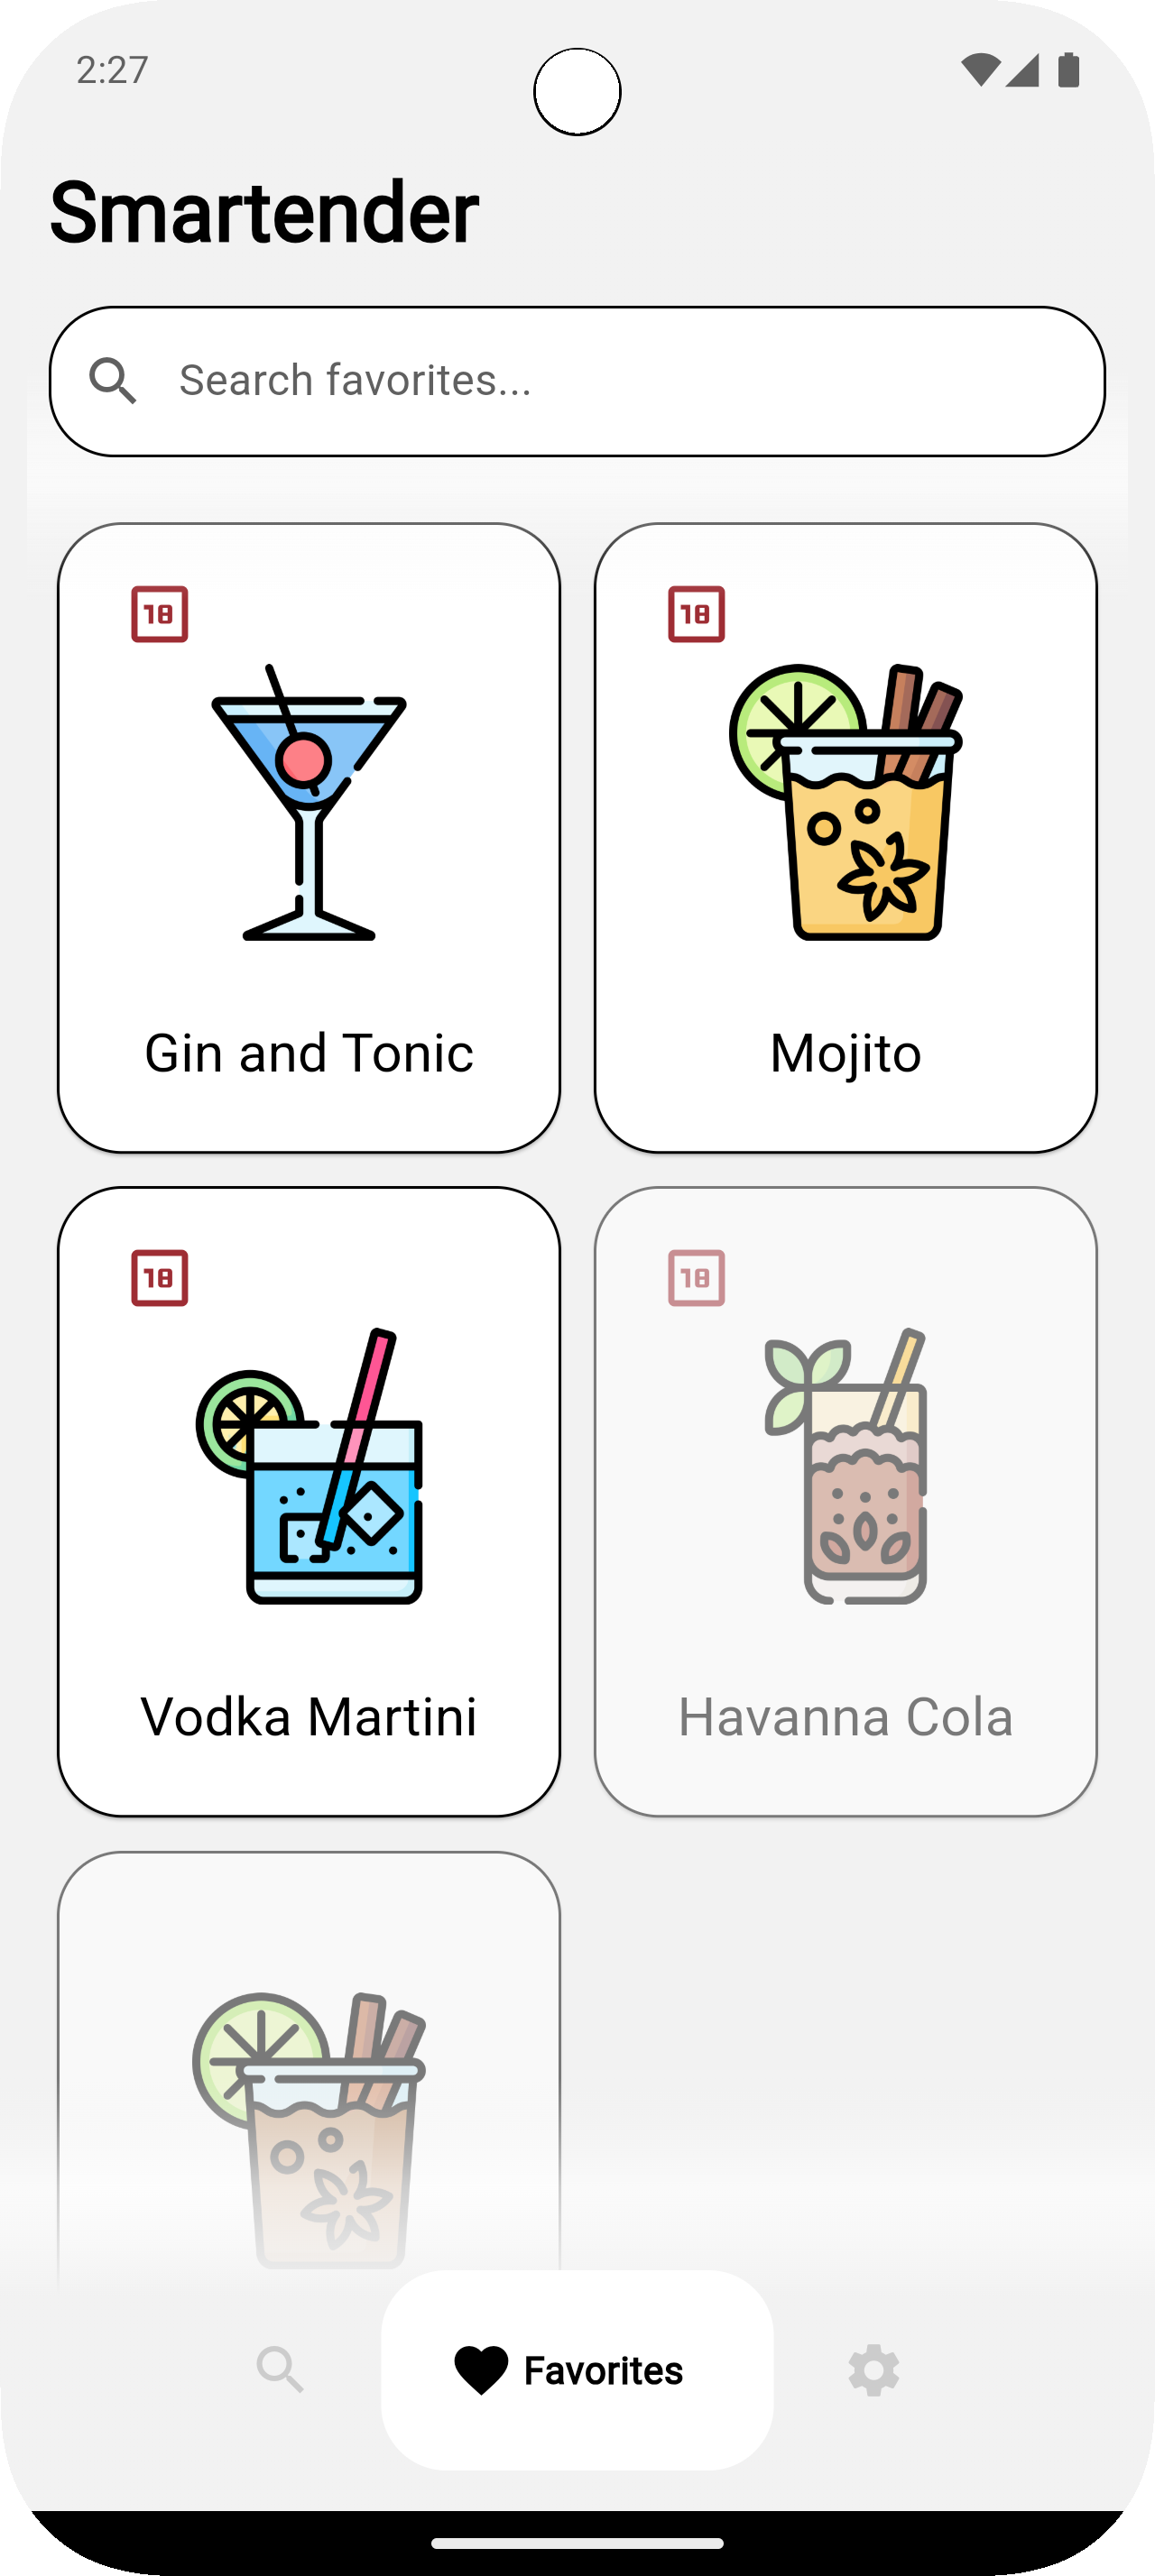
\includegraphics[width=\textwidth]{graphics/images/favorites_light.png}
        \caption{Favoritenansicht im Lightmode}
        \label{fig:favorites_light}
    \end{minipage}
    \hfill
    \begin{minipage}{0.27\textwidth}
        \centering
        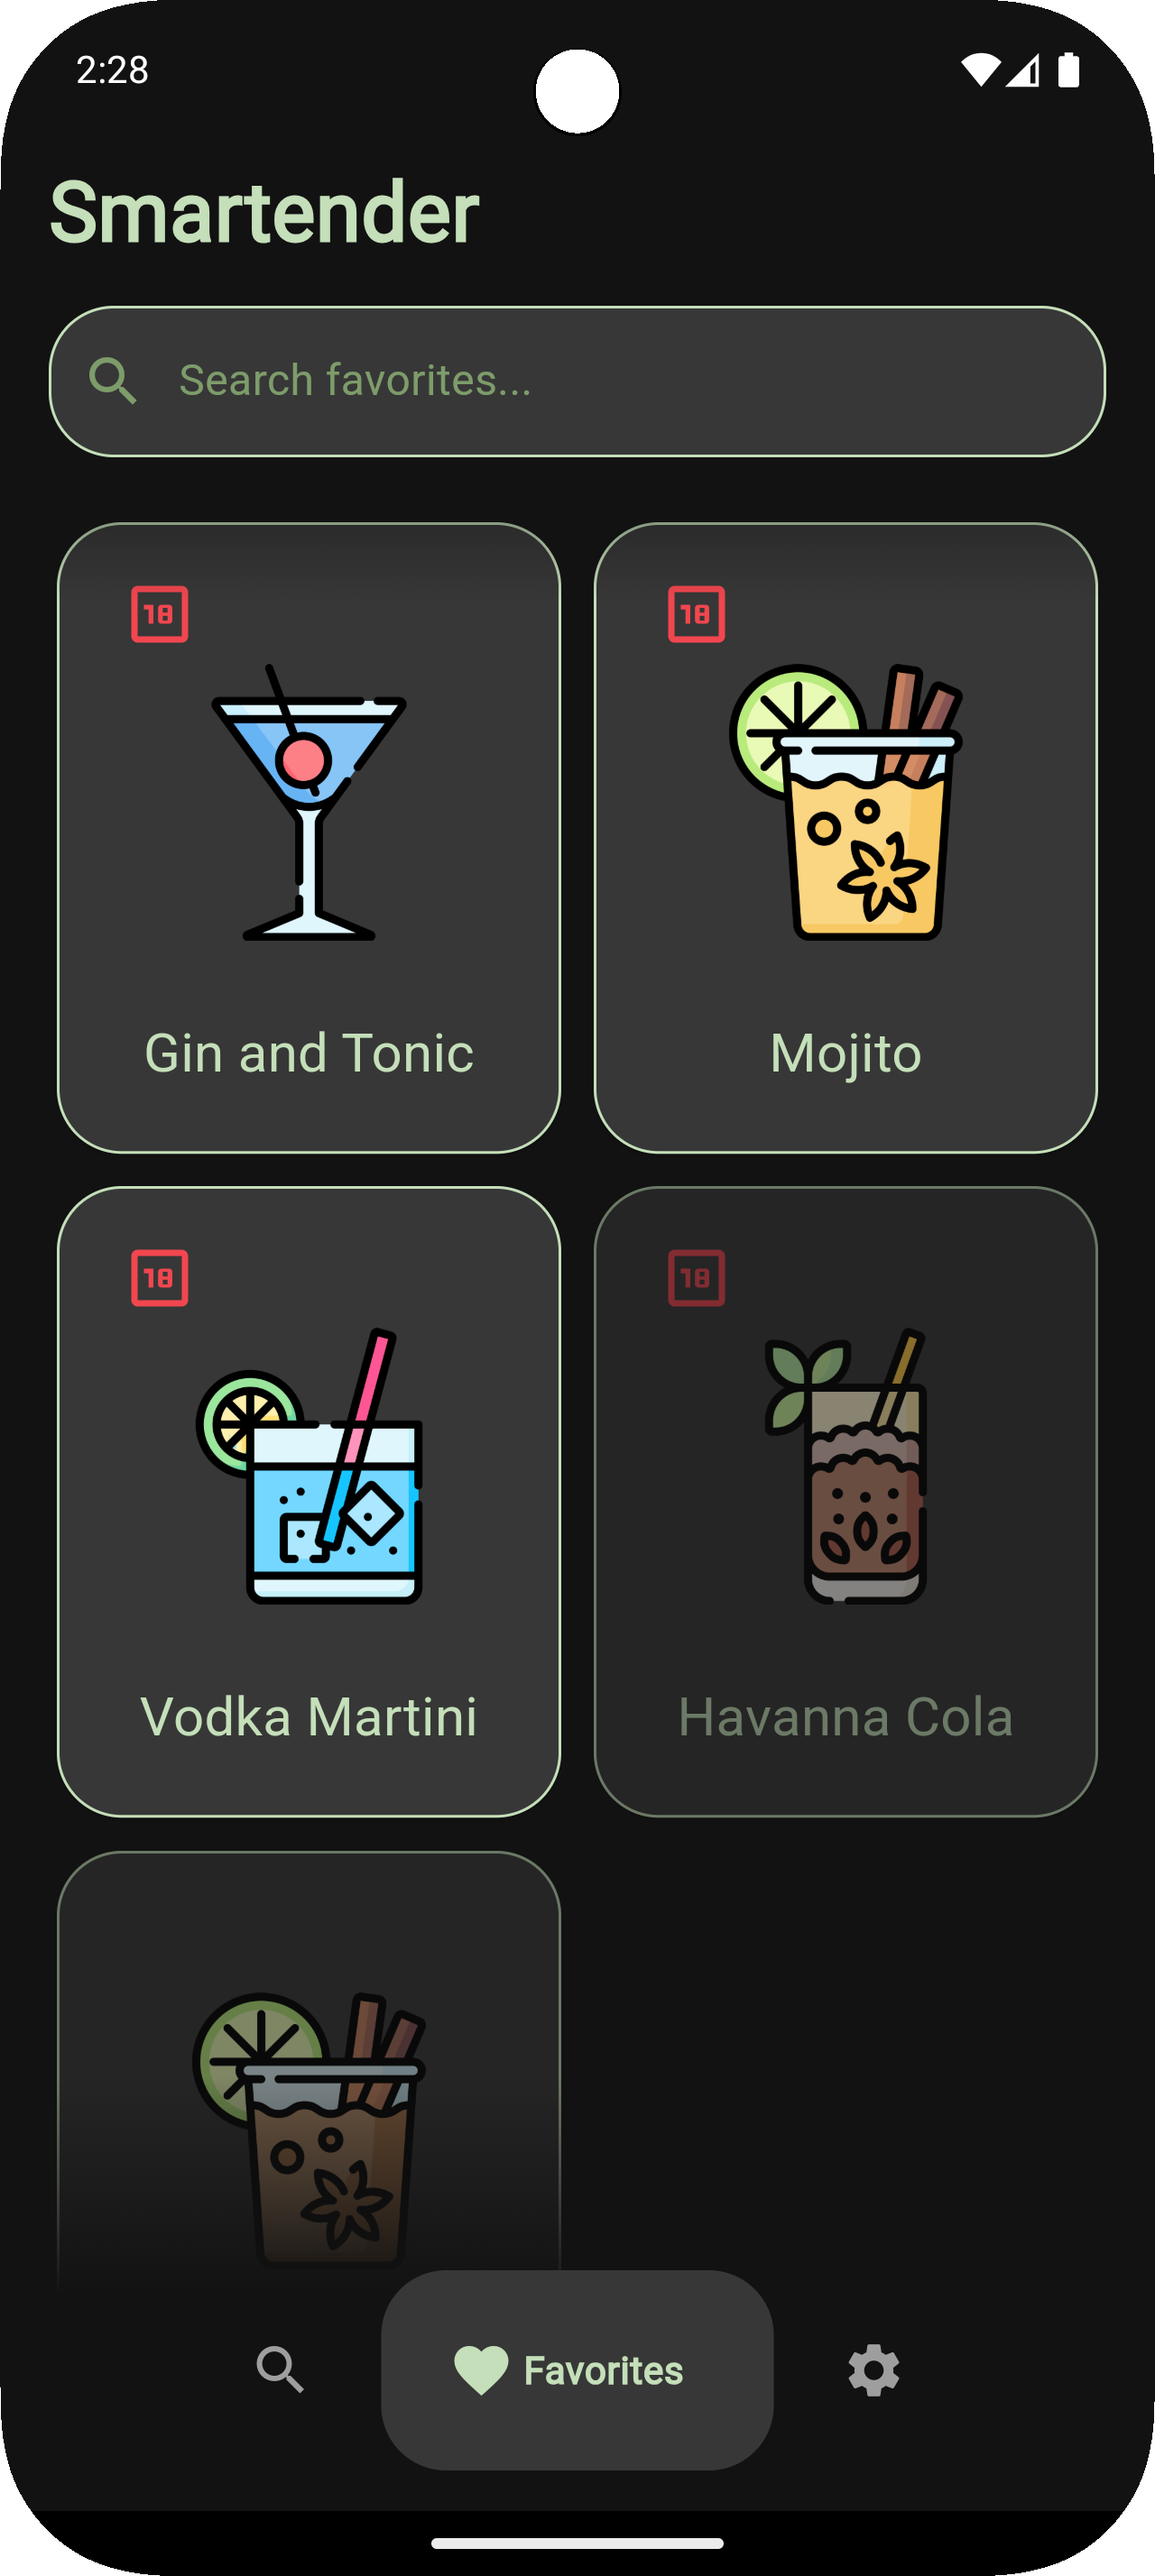
\includegraphics[width=\textwidth]{graphics/images/favorites_dark.png}
        \caption{Favoritenansicht im Darkmode}
        \label{fig:favorites_dark}
    \end{minipage}
    \hfill
    \begin{minipage}{0.27\textwidth}
        \centering
        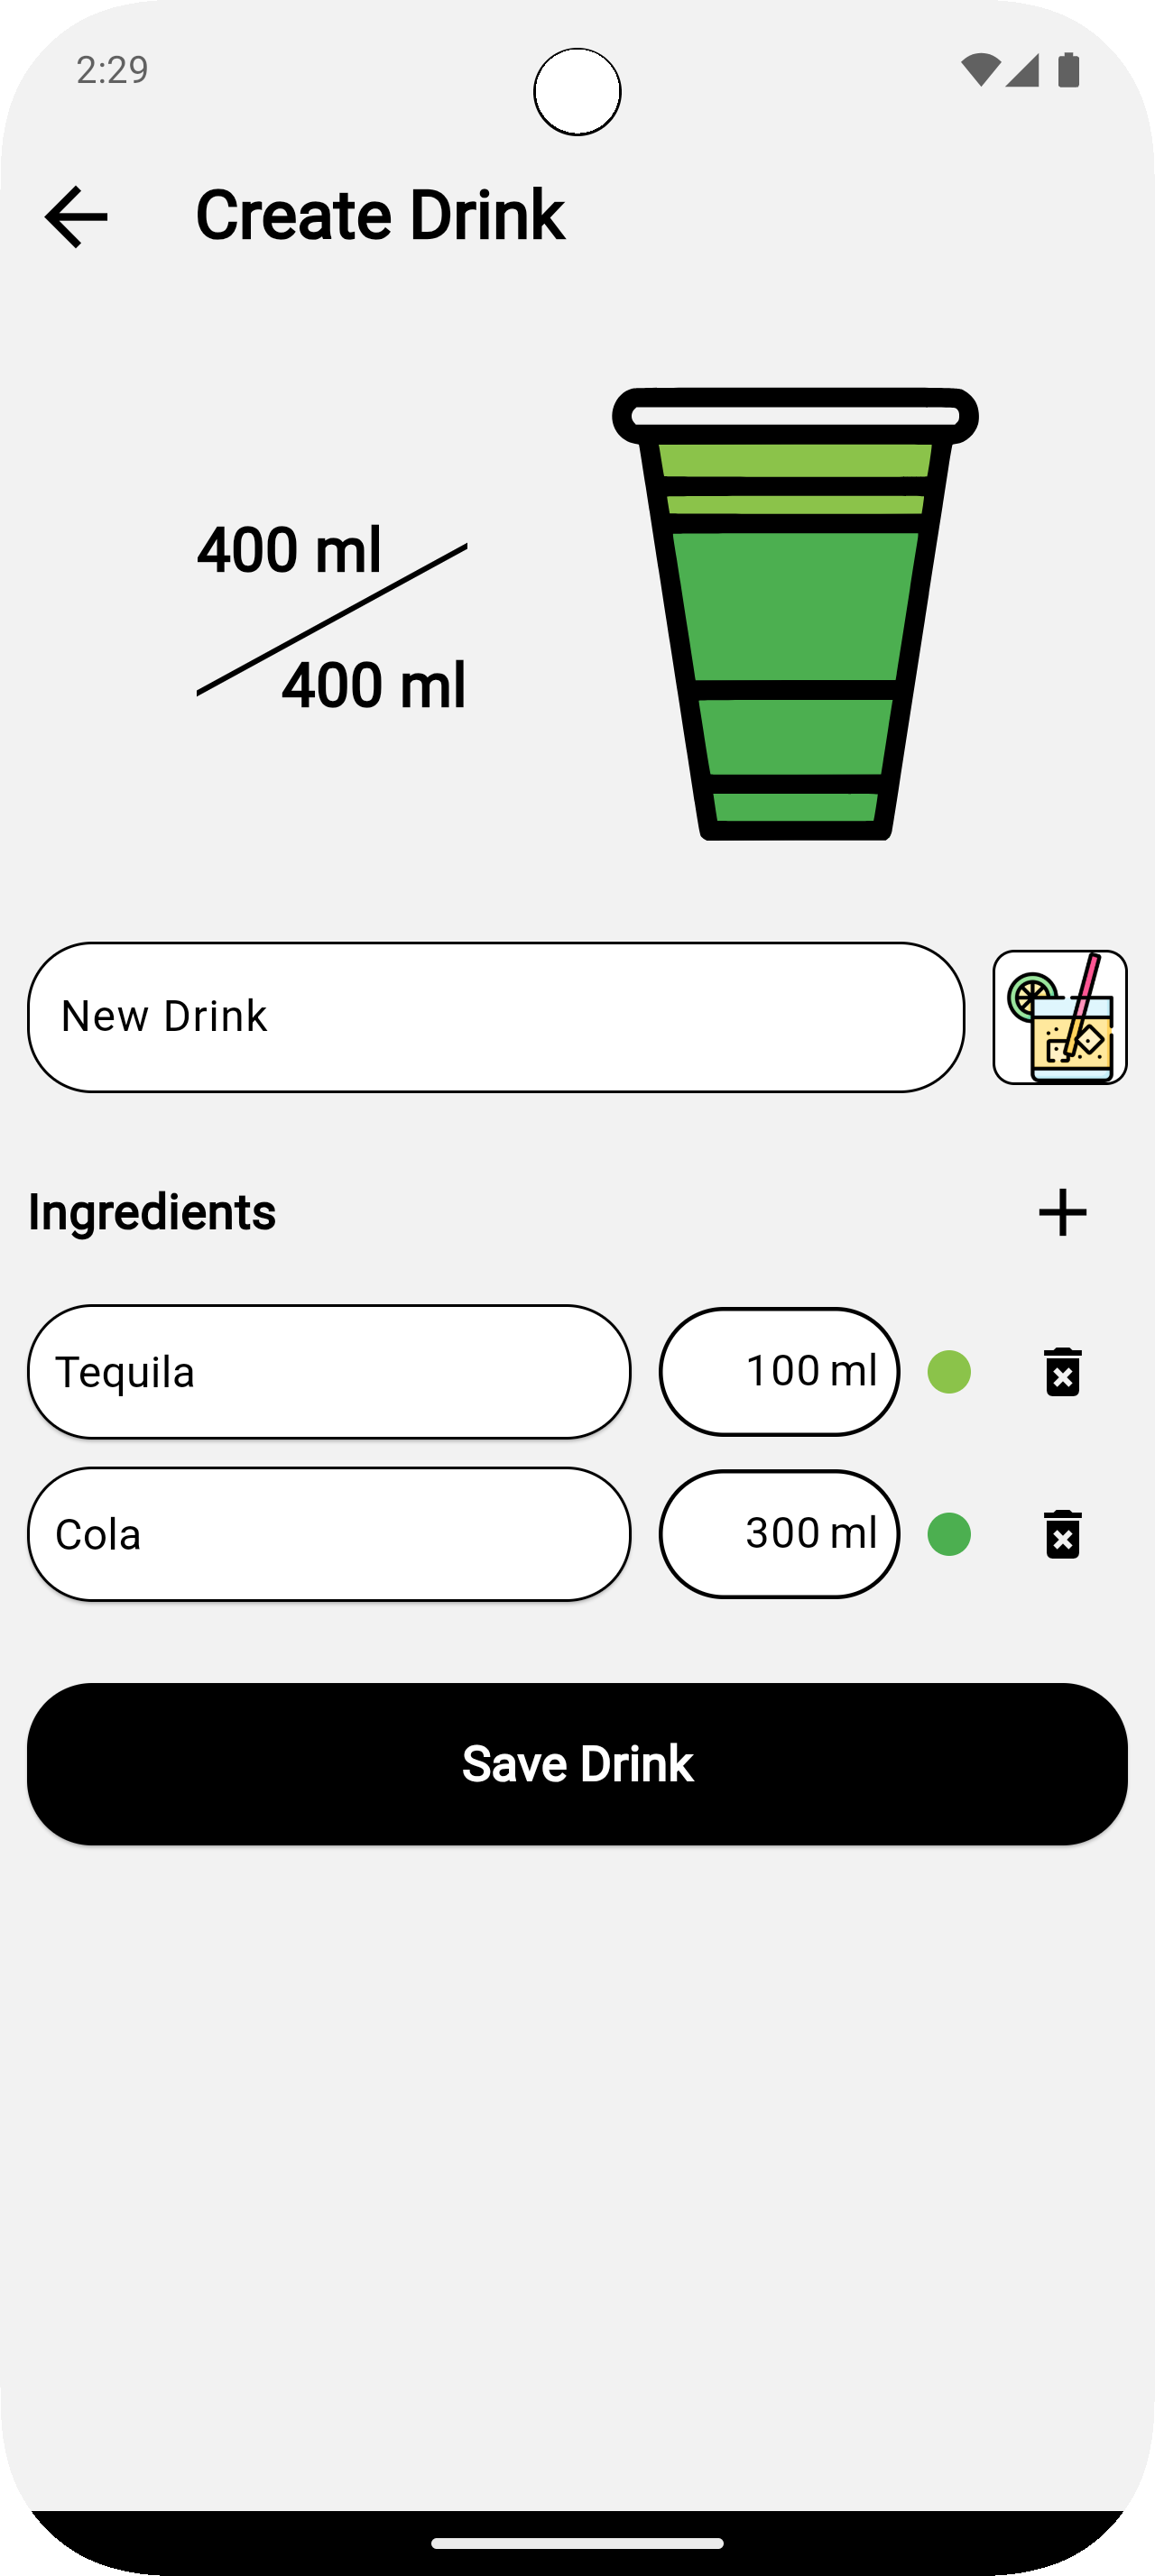
\includegraphics[width=\textwidth]{graphics/images/create_drink.png}
        \caption{Createdrinkscreen im Lightmode}
        \label{fig:create_drink}
    \end{minipage}
    \label{fig:favorites}
\end{figure}



\subsection{Integration und Kommunikation}
Die App kommuniziert über eine REST-API mit dem Backend, wodurch Daten wie Benutzerrezepte, Zutaten und Bestellungen synchronisiert werden. Diese Architektur ermöglicht eine nahtlose Integration und stellt sicher, dass alle Geräte jederzeit auf aktuelle Daten zugreifen können. Die REST-API stellt Endpunkte für folgende Aufgaben bereit:

\begin{itemize}
    \item Abruf und Aktualisierung von Benutzerinformationen
    \item Verwaltung von Rezepten und Zutaten
    \item Auslösen und Überwachung von Bestellungen
\end{itemize}
Eine wichtige Optimierung in der App war die Reduzierung unnötiger Backend-Aufrufe. Ursprünglich wurden Daten alle 10 Sekunden automatisch aktualisiert, was zu einer hohen Serverlast führen konnte. Dies wurde so angepasst, dass die Aktualisierung nur erfolgt, wenn ein Benutzer zwischen den Hauptscreens wechselt. Dadurch konnte die Performance des Systems deutlich verbessert werden.

\subsection{Entwicklungsprozess}
Während der Entwicklung traten einige Herausforderungen auf, insbesondere im Hinblick auf die Anpassung der App an unterschiedliche Bildschirmauflösungen. Obwohl Flutter eine responsive Gestaltung ermöglicht, kam es bei Tests mit einem Samsung S24 Ultra zu einem Overflow-Fehler. Dieser wurde als Einzelfall behandelt, da die App auf anderen Geräten fehlerfrei funktionierte. Zur Entwicklung wurden folgende Tools genutzt:

\begin{itemize}
    \item \textbf{Android Studio:} Hauptentwicklungsumgebung für Android.
    \item \textbf{Postman:} Testen der REST-API-Schnittstellen.
    \item \textbf{Xcode:} Build-Prozess und Tests für iOS-Geräte.
\end{itemize}
Um technische Details zu überprüfen und Designentscheidungen zu bewerten, wurden mehrere Testversionen der App erstellt. Diese wurden unter den Entwicklern getestet, um Fehler zu identifizieren und Verbesserungen vorzunehmen. Dieser iterative Ansatz ermöglichte eine kontinuierliche Optimierung der App.

    
\newpage

\section{Integration und Tests}(4–5 Seiten)
Die Integration und Tests spielten eine zentrale Rolle im Entwicklungsprozess des Projekts, um sicherzustellen, dass die einzelnen Komponenten (App, Backend und Hardware) nahtlos zusammenarbeiten und die gesamte Funktionalität des Cocktailautomaten zuverlässig bereitstellen.

\subsection{Integration der Komponenten}

Die Integration des Gesamtsystems wurde schrittweise durchgeführt. Der Fokus lag darauf, die Kommunikation zwischen der App, dem Backend und der Hardware zu überprüfen und sicherzustellen, dass Bestellungen korrekt verarbeitet und an die Hardware weitergeleitet werden. Im Rahmen des Projekts wurde dabei folgender Prozess verifiziert:

\begin{itemize}
  \item Die mobile App sendet eine Bestellung mit einem Rezept an das Backend.
  \item Das Backend verarbeitet die Bestellung, greift auf die Rezeptdatenbank zu und leitet die relevanten Steuerbefehle an die Hardware weiter.
  \item Die Hardware führt die Befehle aus, steuert die Pumpen und Motoren an und stellt das gewünschte Rezept her.
\end{itemize}

Die Integrationsprüfung umfasste dabei verschiedene Szenarien, einschließlich der Erstellung und Zubereitung mehrerer Testrezepte, wobei aus praktischen Gründen Wasser anstelle der tatsächlichen Zutaten verwendet wurde. Die erfolgreiche Durchführung dieser Tests zeigte, dass die gesamte Prozesskette von der App bis zur Hardware stabil und fehlerfrei funktioniert.

\subsection{Teststrategie}

Im Projekt wurden die Tests ad hoc und iterativ durchgeführt, um Fehler schnell zu identifizieren und zu beheben. Die wichtigsten Tests waren:

\begin{itemize}
  \item \textbf{Integrationstests:} Regelmäßige Überprüfung, ob die gesamte Prozesskette (App \textrightarrow{} Backend \textrightarrow{} Hardware) wie gewünscht funktioniert.
  \item \textbf{Systemtests:} Abschließende Tests, bei denen mehrere Testrezepte angelegt und zubereitet wurden. Diese Tests stellten sicher, dass die Datenübertragung, Rezeptverwaltung und Hardwaresteuerung korrekt umgesetzt sind.
  \item \textbf{Lasttests:} Überprüfung der Systemperformance und Stabilität bei höherer Belastung (siehe Abschnitt \ref{subsec:lasttests}).
  \item \textbf{App-Usability-Tests:} Um die Benutzerfreundlichkeit und Funktionalität der mobilen App zu evaluieren, wurde diese neun Personen vorgestellt. Die Nutzer erhielten die Gelegenheit, alle Funktionen der App zu testen. Anschließend bewerteten sie die App in den Kategorien \textit{Benutzerfreundlichkeit}, \textit{Funktionsumfang} sowie \textit{Stabilität und Leistung} auf einer Skala von 1 (schlecht) bis 5 (sehr gut). Die Ergebnisse waren überwiegend positiv, insbesondere im Bereich Stabilität und Leistung, wo keine Probleme festgestellt wurden. Alle Teilnehmer lobten die intuitive Bedienung und das klare Design.
\end{itemize}

\subsection{Lasttests}
\label{subsec:lasttests}

Um die Skalierbarkeit und Performance des Systems zu überprüfen, wurden Lasttests mithilfe von \texttt{k6} durchgeführt. Die Tests konzentrierten sich auf die Belastbarkeit der Backend-API bei einer großen Anzahl gleichzeitiger Anfragen. Dabei wurden unterschiedliche Szenarien simuliert, darunter das Abrufen von Rezepten und das Auslösen von Bestellungen.\newline

\textbf{Beispiel-Szenario:}
\begin{itemize}
  \item Stufenweise Erhöhung der gleichzeitigen Benutzer von 10 auf 100 in Intervallen von 30 Sekunden.
  \item Messung von Latenzzeiten, Fehlerraten und Erfolgsquoten.
\end{itemize}

\textbf{Herausforderungen:} Während der Tests zeigte sich, dass bei starker Auslastung und mehreren Containerinstanzen Bestellungen nicht immer korrekt verarbeitet wurden. Dies lag daran, dass Websocket-Verbindungen jeweils im RAM der Container gehalten werden. Wenn eine Anfrage an einen anderen Container weitergeleitet wird, als den, der die Verbindung hält, konnte diese nicht verarbeitet werden.\newline

\textbf{Ergebnisse:} Die genaue Analyse der Lasttestergebnisse wird in Abschnitt \ref{subsec:lasttest_results} beschrieben.

\subsection{Fehlerbehebung und Lösungen}

Ein Hauptproblem während der Lasttests war die Verwaltung der Websocket-Verbindungen. Um dieses Problem zu beheben, könnten folgende Maßnahmen zukünftig implementiert werden:

\begin{itemize}
  \item Verwendung eines dedizierten Websocket-Servers, der Verbindungen zentral verwaltet.
  \item Einführung eines Lastverteilers, der Anfragen konsistent an die richtigen Container weiterleitet.
\end{itemize}

Diese Maßnahmen könnten die Zuverlässigkeit und Skalierbarkeit des Systems erheblich verbessern.

    
\newpage

\section{Ergebnisse und Bewertung}(3–4 Seiten)
In diesem Abschnitt werden die erzielten Ergebnisse des Projekts beschrieben und kritisch bewertet. 
Der Fokus liegt auf der funktionalen Umsetzung, der Leistungsbewertung des Systems und einer Analyse 
der Stärken und Schwächen.

\subsection{Funktionale Ergebnisse}

Das Projektziel, einen voll funktionsfähigen Prototypen für einen smarten Cocktailautomaten zu 
entwickeln, wurde erfolgreich erreicht. Die wesentlichen funktionalen Anforderungen konnten 
umgesetzt werden:

\begin{itemize}
  \item \textbf{Automatisierte Cocktailzubereitung:} Die Hardware steuert präzise die \\Pumpen und 
  Motoren, um Zutaten gemäß den Rezeptvorgaben abzugeben.
  \item \textbf{Mobile App:} Benutzer können über eine intuitive App Rezepte erstellen, verwalten 
  und Bestellungen auslösen.
  \item \textbf{Backend-Integration:} Das Backend verarbeitet Bestellungen zuverlässig, 
  \\synchronisiert Benutzerdaten und leitet Steuerbefehle an die Hardware \\weiter.
\end{itemize}

Die abschließenden Integrationstests zeigten, dass das Gesamtsystem von der Rezeptbestellung in der 
App bis zur Zubereitung durch die Hardware stabil \\funktioniert.

\subsection{Lasttestergebnisse und Analyse}

Zur Bewertung der Performance und Skalierbarkeit des Systems wurden umfassende Lasttests mit dem 
Tool \texttt{k6} durchgeführt. Diese Tests simulierten eine Vielzahl gleichzeitiger 
Benutzeranfragen, um Engpässe und Optimierungspotenziale zu identifizieren. Die wichtigsten 
Ergebnisse sind im Folgenden zusammengefasst.

\subsubsection*{Gesamtergebnisse}

\subsubsection*{Wichtige Metriken}
\begin{itemize}
    \item \textbf{Gesamtanfragen:} 16.506
    \item \textbf{Fehlerrate:} 0,08\% (14 fehlgeschlagene Anfragen)
    \item \textbf{Durchschnittliche Antwortzeit:} 274,48 ms
    \item \textbf{Minimale Antwortzeit:} 13,87 ms
    \item \textbf{Median der Antwortzeit:} 19,75 ms
    \item \textbf{Maximale Antwortzeit:} 282.415,99 ms
    \item \textbf{90. Perzentil der Antwortzeit:} 78,66 ms
    \item \textbf{95. Perzentil der Antwortzeit:} 121,84 ms
\end{itemize}

% ERFOLGSRATE --------------------------------------------------------------------------------------
\subsubsection*{Erfolgsrate}

\begin{table}[H]
    \centering
    % \resizebox{\textwidth}{!}{%
        \begin{tabular}{|l|r|r|r|}
            \hline
            \textbf{Test} & \textbf{Erfolgreich} & \textbf{Fehlgeschlagen} & \textbf{Erfolgsrate} \\
            \hline
            Nutzerregistrierung   &  263 &   0 &  100\% \\
            Nutzer einloggen      &  263 &   0 &  100\% \\
            Hardwareregistrierung &  262 &   1 &   99\% \\
            Drink erstellen       & 2615 &   5 &   99\% \\
            Slot setzen           & 1304 &   6 &   99\% \\
            Rezept erstellen      & 2619 &   1 &   99\% \\
            Zutat hinzufügen      & 2620 &   0 &  100\% \\
            Favorit erstellen     &  785 &   1 &   99\% \\
            Slots abfragen        &  262 &   0 &  100\% \\
            Favoriten abfragen    &  263 &   0 &  100\% \\
            \hline
        \end{tabular}
    % }
    \caption{Tests je Endpunkt und Erfolgsrate}
    \label{tab:test_success_rate}    
\end{table}

Die Erfolgsrate der einzelnen API-Endpunkte ist insgesamt hoch. Die Nutzerregistrierung und das 
Einloggen waren zu 100\% erfolgreich, während die Hardwareregistrierung eine Erfolgsrate von 99\% 
aufweisen. Die Fehlerrate bei der Erstellung von Getränken und Rezepten, dem setzen von Slots und 
dem hinzufügen von Bestandteilen zu einem Rezept liegt bei 1\%. Diese Fehler lassen sich aber 
allesamt durch das Fehlschlagen der Hardwareregistrierung erklären, da diese für einen Eintrag in 
die Datenbank benötigt wird. Die Erfolgsrate der Favoritenfunktion liegt aus dem selben Grund 
lediglich bei 99\%. Alles in allem sind die Ergebnisse zufriedenstellend. 
Das scheitern der Hardware registrieren Anfrage ist auf eine Auslastung der Container Instanz 
zurückzuführen, und könnte mit mehr Leistung, mit weiteren Container Instanzen oder einer 
Optimierung der Anfrage behoben werden.

% ANTOWRTZEITEN ------------------------------------------------------------------------------------
\subsubsection*{Antwortzeiten pro Endpunkt}

Die Antwortzeiten für spezifische API-Endpunkte zeigen deutliche Unterschiede, die auf 
unterschiedliche Verarbeitungskomplexität hinweisen. Die wichtigsten Werte sind in Tabelle 
\ref{tab:response_times} dargestellt.

\begin{table}[H] 
    \centering
    % \resizebox{\textwidth}{!}{%
        \begin{tabular}{|l|r|r|r|r|}
            \hline
            \textbf{Endpunkt} &
            \textbf{Durchschnitt} & 
            \textbf{Median} & 
            \textbf{90. Perzentil} & 
            \textbf{Max} \\
            \hline
            Nutzer registrieren     &  145,60 & 102,70 & 219,23 &   1224,98 \\
            Nutzer einlogen         &  155,90 & 102,51 & 283,79 &   1530,31 \\
            Hardware registrieren   & 1241,48 &  70,54 & 218,08 & 282415,99 \\
            Drink erstellen         &  588,13 &  19,39 &  52,83 & 282275,98 \\
            Rezept erstellen        &  136,98 &  19,10 &  42,42 & 282282,60 \\
            Zutat hinzufügen        &   29,39 &  18,85 &  46,66 &    422,70 \\
            Slot setzen             & 1341,94 &  23,35 &  79,69 & 282292,87 \\
            Rezept favorisieren     &  268,85 &  24,01 &  64,44 & 183405,20 \\
            Alle Favoriten abfragen &   29,58 &  20,01 &  51,67 &    227,09 \\
            Slotbelegung abfragen   &   64,92 &  48,96 & 112,32 &    355,33 \\
            \hline
        \end{tabular}
    % }
    \caption{Antwortzeiten je Endpunkt in Millisekunden}
    \label{tab:response_times}
\end{table}

Bei einer genaueren Betrachtung der Antwortzeiten pro Endpunkt fällt auf, dass die Endpunkte mit 
den höchsten Maximalwerten (Hardware registrieren, Drink erstellen, Rezept erstellen, Slot setzen, 
Favorit setzen) wieder die selben Punkte sind welche bereits zuvor als fehleranfällig identifiziert
wurden. Die Antwortzeiten sind in diesen Fällen sehr hoch, was auf eine Überlastung der Container 
Instanz zurückzuführen ist. Die Antwortzeiten der anderen Endpunkte sind im Vergleich dazu sehr
gering. Die Antwortzeiten der Endpunkte Zutat hinzufügen, Alle Favoriten abfragen und Slotbelegung
abfragen sind besonders niedrig, was auf eine geringe Verarbeitungskomplexität hinweist.

% USABILITY ----------------------------------------------------------------------------------------
\subsection{User-Test Ergebnisse}

Zur Evaluation der Benutzerfreundlichkeit, des Funktionsumfangs und der Stabilität der mobilen App 
wurden neun Personen eingeladen, die App zu testen. Sie bewerteten die App in den drei Kategorien 
auf einer Skala von 1 (schlecht) bis 5 (sehr gut). Die Ergebnisse sind in Tabelle 
\ref{tab:user_tests} und in der Visualisierung in Abbildung \ref{fig:user_tests2} dargestellt.

\begin{table}[h!]
    \centering
    \begin{tabular}{|l|c|}
        \hline
        \textbf{Kategorie} & \textbf{Durchschnittliche Bewertung} \\
        \hline
        Benutzerfreundlichkeit & 4,44 \\
        Funktionsumfang & 4,22 \\
        Stabilität und Leistung & 4,88 \\
        \hline
    \end{tabular}
    \caption{Ergebnisse der Benutzerbewertungen}
    \label{tab:user_tests}
\end{table}

\clearpage
\begin{figure}[h!]
    \centering
    \begin{minipage}{0.80\textwidth}
        \centering
        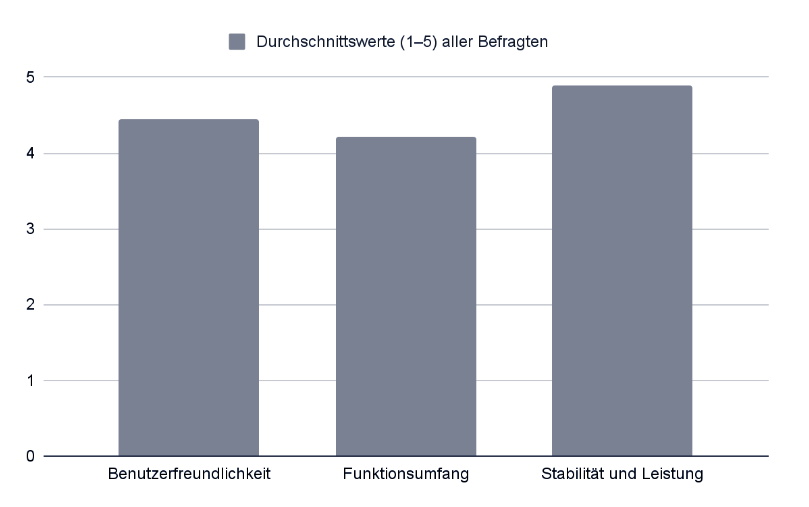
\includegraphics[width=\textwidth]{graphics/images/usertests_app.png}
        \caption{Usertest}
        \label{fig:user_tests2} % Direkt nach der caption setzen
    \end{minipage}
\end{figure}


\hyphenation{Live-Umgebung}
\hyphenation{Web-socket-Ver-bind-ung}
Die Tests haben gezeigt, dass das System in einer Live-Umgebung grundsätzlich stabil arbeitet. 
Allerdings wurden Skalierungsprobleme bei Websocket-Verbindungen identifiziert, die durch eine 
zentrale Verwaltung oder eine konsistente Lastverteilung gelöst werden könnten. Die meisten API-
Endpunkte zeigten zufriedenstellende Antwortzeiten und Erfolgsquoten. Die Schwachstellen bieten 
jedoch Anknüpfungspunkte für zukünftige Optimierungen.

\subsection{Stärken und Schwächen}

\subsubsection{Stärken}

Das Projekt weist folgende Stärken auf:
\begin{itemize}
  \item \textbf{Benutzerfreundlichkeit:} Die App bietet eine intuitive Benutzeroberfläche und 
  ermöglicht eine einfache Verwaltung von Rezepten und Geräten.
  \item \textbf{Technische Umsetzung:} Die Kombination aus App, Backend und Hardware zeigt das 
  Potenzial von IoT-Technologien in Smart-Home-Umgebungen.
  \item \textbf{Modularität:} Die Architektur des Systems ermöglicht zukünftige Erweiterungen, z. B. 
  die Integration zusätzlicher Geräte oder neue Funktionen.
\end{itemize}

\subsubsection*{Schwächen}

Einige Schwächen des aktuellen Prototyps wurden identifiziert:
\begin{itemize}
  \item \textbf{Skalierbarkeit:} Die Verwaltung von Websocket-Verbindungen in einer 
  containerisierten Umgebung führte bei hoher Last zu Problemen.
  \item \textbf{Fehlende Tests:} Es wurden keine umfassenden automatisierten Tests für die einzelnen 
  Systemkomponenten implementiert.
  \item \textbf{Hardware:} Obwohl die Hardware zuverlässig arbeitet, könnten Optimierungen in der 
  Dosiergenauigkeit und Stabilität vorgenommen werden.
\end{itemize}

\subsection{Zusammenfassung der Ergebnisse}

Das Projekt hat gezeigt, dass IoT-Technologien erfolgreich zur Automatisierung von Alltagsaufgaben 
eingesetzt werden können. Die entwickelten Systeme arbeiten zuverlässig und erfüllen die definierten 
funktionalen Anforderungen. Gleichzeitig wurden Schwächen aufgedeckt, die als Grundlage für 
zukünftige Optimierungen dienen können.

\subsection{Empfehlungen}
\hyphenation{Web-socket-Ser-ver}
Auf Basis der Testergebnisse und identifizierten Schwächen werden folgende Maßnahmen für zukünftige 
Verbesserungen empfohlen:
\begin{itemize}
  \item \textbf{Optimierung der Skalierung:} Einführung eines zentralen Websocket-Servers oder 
  konsistenter Lastverteilung, um Kommunikationsprobleme bei hoher Last zu beheben.
  \item \textbf{Automatisierte Tests:} Entwicklung und Implementierung umfassender \\
  Unit- und Integrationstests.
  \item \textbf{Hardware-Optimierungen:} Verbesserung der Dosiergenauigkeit und Integration 
  zusätzlicher Sensorik zur Überwachung.
\end{itemize}

% BOXPLOT PUMPEN -----------------------------------------------------------------------------------
\newpage
\begin{figure}[h!]
    \centering
    \begin{tikzpicture}
        \begin{axis}[
            boxplot/draw direction=y,
            ylabel={ Menge in Milliliter }, % Beschriftung der y-Achse
            xlabel={ Pumpen }, % Beschriftung der x-Achse
            xtick={ 1, 2, 3, 4, 5, 6 }, % Positionen der xticks
            xticklabels={ 1, 2, 3, 4, 5, 6 }, % Labels der xticks
            ymin=210, 
            ymax=430, % Begrenzung der y-Achse
            boxplot/every box/.style={solid}
        ]
        \addplot [
            thick, dashed, blue,
            domain=0:7, % Definiert den Bereich der x-Achse
        ] {400};
        \addplot+ [
            boxplot,
            fill=red4,
            draw=red7,
            solid
        ] table[row sep=\\, y index=0] {
            370 \\ 375 \\ 357 \\ 364 \\ 358 \\ 362 \\ 382 \\ 383 \\ 370 \\ 366 \\ 370 \\ 368 \\ 
            383 \\ 373 \\ 360 \\ 355 \\ 373 \\ 381 \\ 356 \\ 349 \\ 362 \\ 370 \\ 369 \\ 361 \\
        };
        \addplot+ [
            boxplot,
            fill=red4,
            draw=red7,
            solid
        ] table[row sep=\\, y index=0] {
            399 \\ 388 \\ 395 \\ 395 \\ 399 \\ 409 \\ 402 \\ 400 \\ 386 \\ 401 \\ 400 \\ 400 \\ 
            404 \\ 387 \\ 405 \\ 400 \\ 400 \\ 390 \\ 388 \\ 400 \\ 400 \\ 399 \\ 405 \\ 399 \\
        };
        \addplot+ [
            boxplot,
            fill=red4,
            draw=red7,
            solid
        ] table[row sep=\\, y index=0] {
            397 \\ 402 \\ 395 \\ 398 \\ 400 \\ 400 \\ 395 \\ 400 \\ 402 \\ 400 \\ 399 \\ 408 \\ 
            395 \\ 388 \\ 403 \\ 400 \\ 402 \\ 400 \\ 408 \\ 388 \\ 396 \\ 408 \\ 397 \\ 390 \\
        };
        \addplot+ [
            boxplot,
            fill=red4,
            draw=red7,
            solid
        ] table[row sep=\\, y index=0] {
            411 \\ 400 \\ 398 \\ 399 \\ 400 \\ 408 \\ 408 \\ 415 \\ 400 \\ 386 \\ 393 \\ 390 \\ 
            400 \\ 404 \\ 400 \\ 406 \\ 409 \\ 400 \\ 403 \\ 396 \\ 406 \\ 407 \\ 405 \\ 396 \\
        };
        \addplot+ [
            boxplot,
            fill=red4,
            draw=red7,
            solid
        ] table[row sep=\\, y index=0] {
            267 \\ 259 \\ 305 \\ 242 \\ 306 \\ 315 \\ 313 \\ 287 \\ 266 \\ 300 \\ 298 \\ 260 \\ 
            285 \\ 251 \\ 283 \\ 243 \\ 266 \\ 263 \\ 255 \\ 278 \\ 241 \\ 255 \\ 315 \\ 280 \\
        };
        \addplot+ [
            boxplot,
            fill=red4,
            draw=red7,
            solid
        ] table[row sep=\\, y index=0] {
            382 \\ 385 \\ 387 \\ 382 \\ 390 \\ 386 \\ 390 \\ 377 \\ 393 \\ 388 \\ 383 \\ 398 \\
        };
        \end{axis}

    \end{tikzpicture}
    \caption{Pumpenleistung für 400ml}
    \label{fig:pump_performance}
\end{figure}
\newpage
% --------------------------------------------------------------------------------------------------
% --------------------------------------------------------------------------------------------------
% --------------------------------------------------------------------------------------------------
% --------------------------------------------------------------------------------------------------
% --------------------------------------------------------------------------------------------------

\section*{Schlussfolgerungen}
Die Ergebnisse zeigen, dass:
\begin{itemize}
    \item Die Benutzerregistrierung und Rezeptverwaltung besonders fehleranfällig sind (nur 9\% 
        Erfolgsquote).
    \item Die API insgesamt eine hohe Fehlerrate von 45,11\% aufweist, was auf Skalierungs- oder 
        Ressourcenprobleme hindeuten könnte.
    \item Die durchschnittliche Antwortzeit (66,26 ms) akzeptabel ist, aber in Spitzenzeiten (max. 
        644 ms) stark ansteigt.
\end{itemize}

\section*{Empfehlungen}
\begin{itemize}
    \item Optimieren Sie die Ressourcen- und Skalierungseinstellungen von Google Cloud Run.
    \item Reduzieren Sie die Last in der Benutzerregistrierung durch bessere Datenbankabfragen 
        oder asynchrone Prozesse.
    \item Testen Sie kleinere Benutzergruppen, um die Schwellenwerte für Stabilitätsprobleme zu 
        identifizieren.
\end{itemize}

\newpage

\section{Fazit und Ausblick}(2 Seiten)
% Hier folgt der Inhalt des Abschnitts "Fazit und Ausblick".    
\newpage

\section{Anhang}(variabel)
% Hier folgt der Inhalt des Abschnitts "Anhang".

\subsection{Pinbelegung}

\begin{figure}[ht]
  \centering
  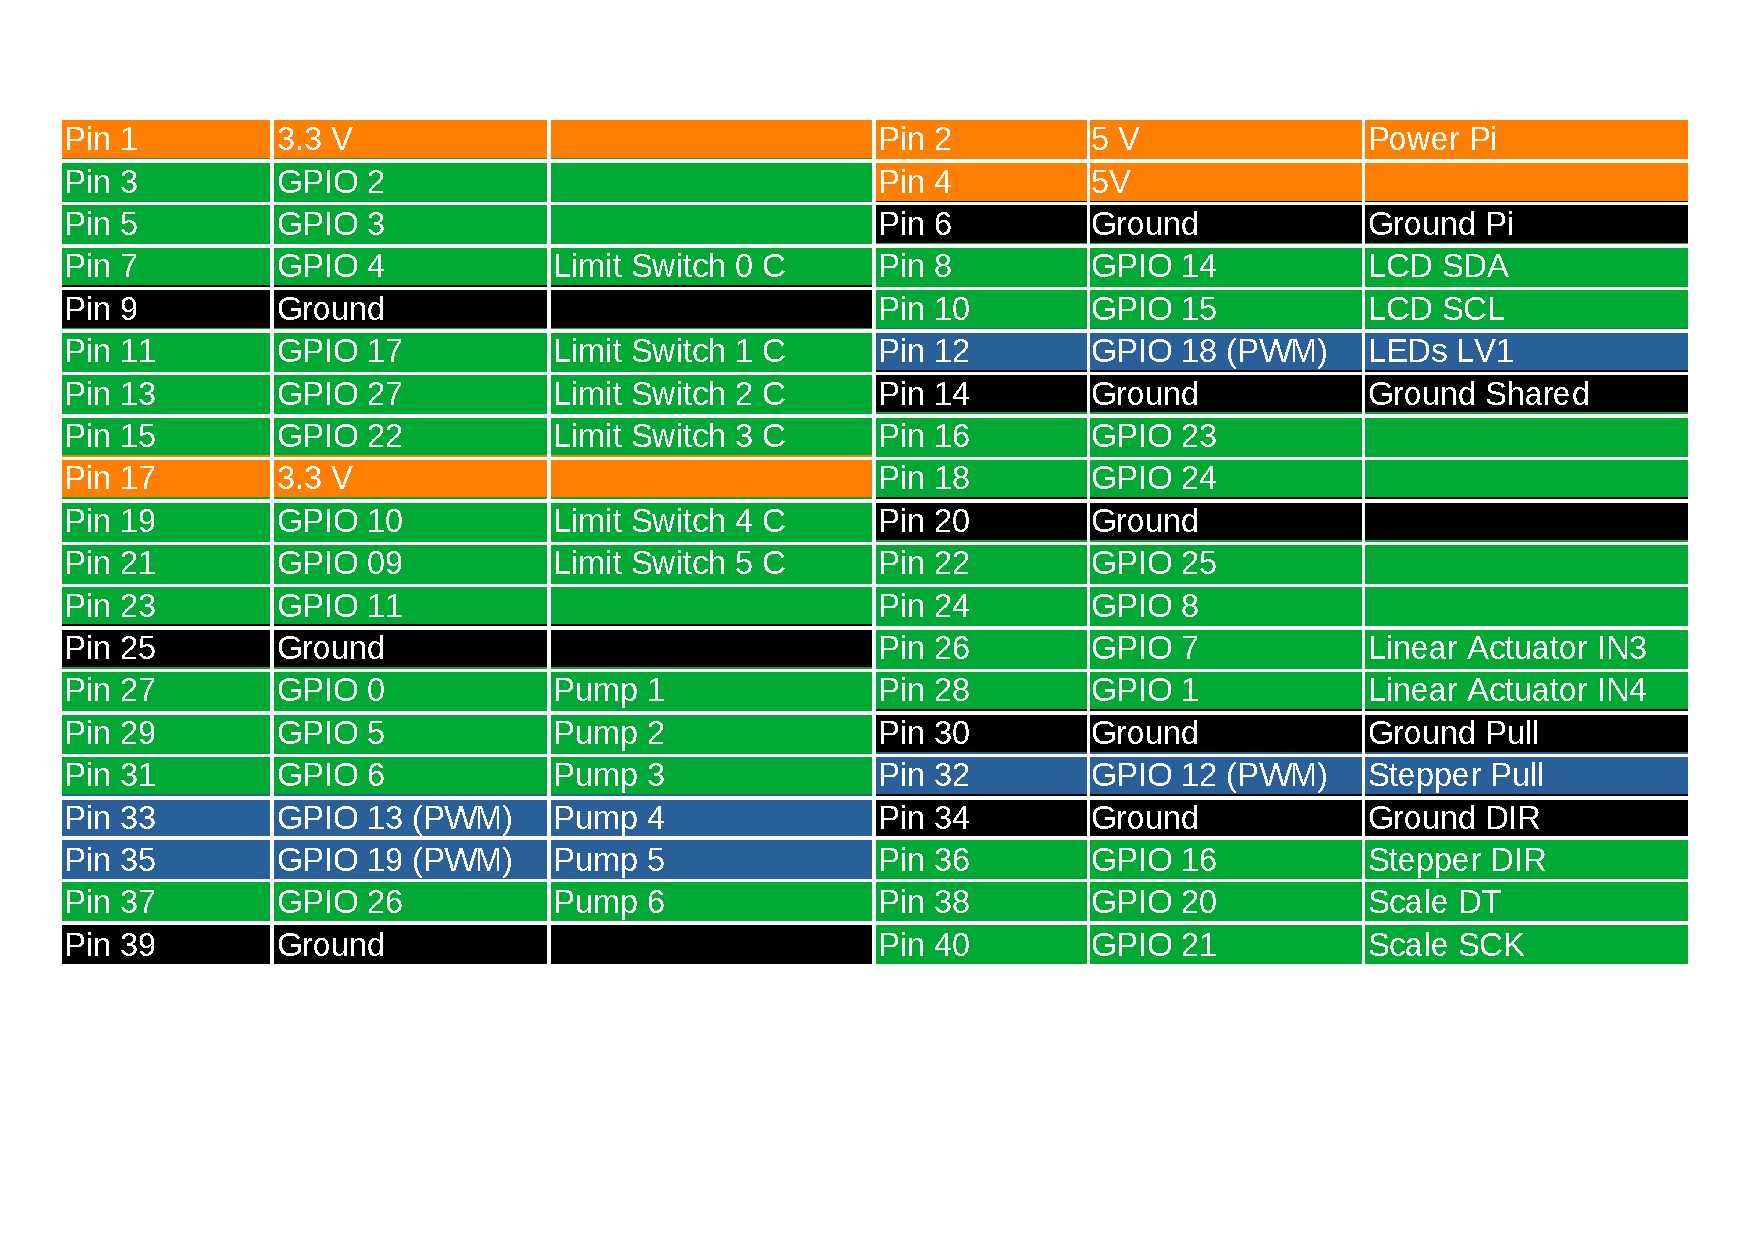
\includegraphics[width=\textwidth]{graphics/images/pinning_final.pdf} % PDF-Datei einfügen
  \caption{Pinbelegung des Rapsberry Pi Zero 2 W}
  \label{fig:pinning}
\end{figure}

\newpage

\subsection{Schaltplan}

\begin{figure}[ht]
  \centering
  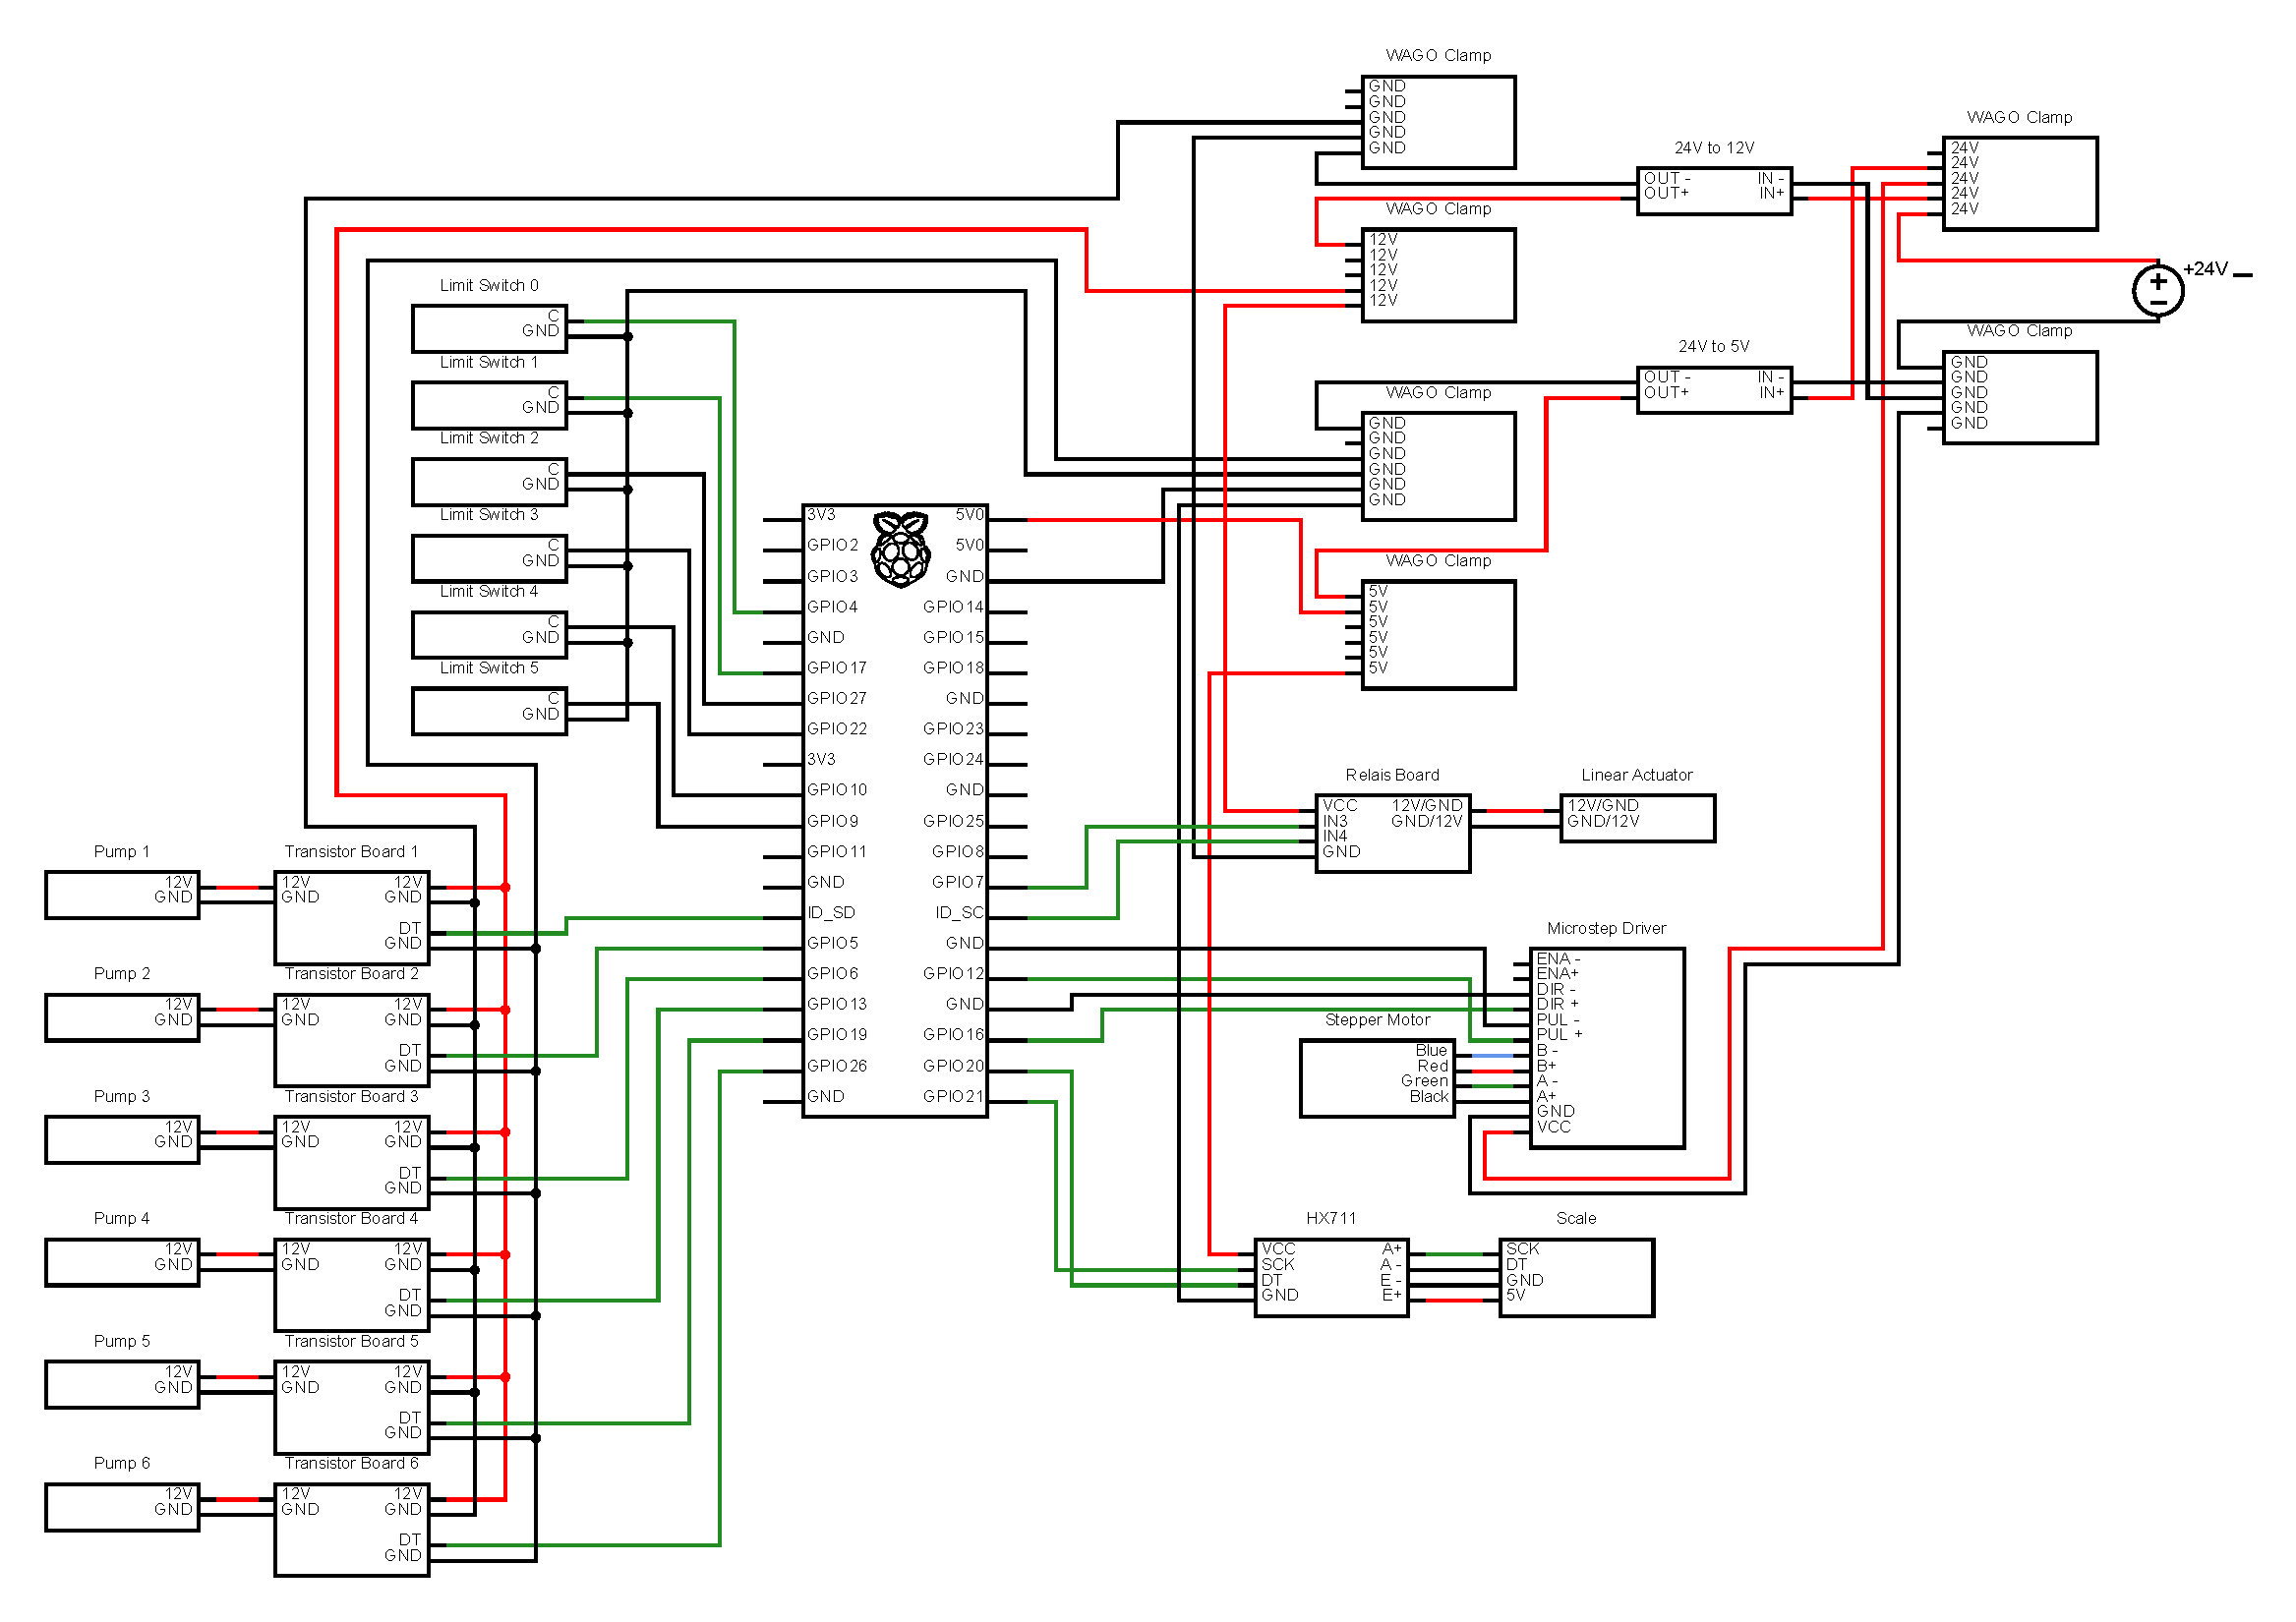
\includegraphics[width=\textwidth]{graphics/images/schaltplan.pdf} % Seite 2 der PDF einfügen
  \caption{Schaltplan der Hardwarekomponenten}
  \label{fig:schaltplan}
\end{figure}

\newpage

\subsection{k6 Testskript}
\begin{lstlisting}[language=JavaScript]
  import http from 'k6/http';
  import { check, sleep } from 'k6';
  import { Counter } from 'k6/metrics';
  
  export let errorCounter = new Counter('errors');
  
  export const options = {
    stages: [
      { duration: '1m', target: 1 }, // 1 Nutzer
      { duration: '1m', target: 2 }, // 2 Nutzer
      { duration: '1m', target: 4 }, // 4 Nutzer
      { duration: '1m', target: 5 }, // 5 Nutzer
      { duration: '1m', target: 20 }, // 20 Nutzer
    ],
  };
  
  const BASE_URL = 'https://smartender-432708816033.europe-west3.run.app';
  const API_KEY = 'b0ec1aa3-98bd-434d-b6b6-f72b99383859';
  
  function randomString(length) {
    const chars = 'abcdefghijklmnopqrstuvwxyz1234567890';
    let result = '';
    for (let i = 0; i < length; i++) {
      result += chars.charAt(Math.floor(Math.random() * chars.length));
    }
    return result;
  }
  
  function generateMacAddress() {
    const hex = '0123456789ABCDEF';
    let mac = [];
    for (let i = 0; i < 6; i++) {
      mac.push(
        hex.charAt(Math.floor(Math.random() * 16)) + hex.charAt(Math.floor(Math.random() * 16))
      );
    }
    return mac.join(':');
  }
  
  export default function () {
    // 1. Registrierung
    const username = `user_${randomString(8)}`;
    const password = 'Password123!';
    const email = `${username}@example.com`;
  
    let registerRes = http.post(
      `${BASE_URL}/api/auth/register`,
      JSON.stringify({
        username,
        password,
        email,
      }),
      {
        headers: { 'Content-Type': 'application/json', 'X-API-Key': API_KEY },
      }
    );
  
    check(registerRes, { 'User registration successful': (res) => res.status === 201 });
    if (registerRes.status !== 201) return;
  
    // 2. Login
    let loginRes = http.post(
      `${BASE_URL}/api/auth/login`,
      JSON.stringify({
        username,
        password,
      }),
      {
        headers: { 'Content-Type': 'application/json', 'X-API-Key': API_KEY },
      }
    );
  
    check(loginRes, { 'User login successful': (res) => res.status === 200 });
    if (loginRes.status !== 200) return;
  
    const loginData = JSON.parse(loginRes.body);
    const jwt = loginData.token;
    const userId = parseInt(loginData.userID);
  
    // 3. Hardware registrieren
    //
    let hardwareRes = http.post(
      `${BASE_URL}/smartender/register`,
      JSON.stringify({
        hardware_name: `Hardware_${randomString(5)}`,
        mac_address: generateMacAddress(),
        user_id: userId,
      }),
      {
        headers: {
          'X-API-Key': API_KEY,
          Authorization: `Bearer ${jwt}`,
        },
      }
    );
  
    check(hardwareRes, { 'Hardware registration successful': (res) => res.status === 200 });
    const hardwareData = JSON.parse(hardwareRes.body);
    const hardwareId = hardwareData.hardwareID;
  
    // 4. Drinks anlegen
    let drinks = [];
    for (let i = 0; i < 10; i++) {
      let drinkRes = http.post(
        `${BASE_URL}/api/user/hardware/${hardwareId}/drinks`,
        JSON.stringify({
          drink_name: `Drink_${randomString(5)}`,
          is_alcoholic: Math.random() > 0.5,
        }),
        {
          headers: {
            'Content-Type': 'application/json',
            'X-API-Key': API_KEY,
            Authorization: `Bearer ${jwt}`,
          },
        }
      );
  
      check(drinkRes, { 'Drink creation successful': (res) => res.status === 201 });
      if (drinkRes.status === 201) drinks.push(JSON.parse(drinkRes.body));
    }
  
    // 5. Slots befuellen
    for (let i = 0; i < Math.min(drinks.length, 5); i++) {
      let setSlotRes = http.put(
        `${BASE_URL}/api/user/hardware/${hardwareId}/slots/${i + 1}`,
        JSON.stringify({
          drink_id: drinks[i].drink_id,
        }),
        {
          headers: {
            'Content-Type': 'application/json',
            'X-API-Key': API_KEY,
            Authorization: `Bearer ${jwt}`,
          },
        }
      );
  
      check(setSlotRes, { 'Slot set successfully': (res) => res.status === 204 });
    }
  
    // 6. Rezepte anlegen
    let recipes = [];
    for (let i = 0; i < 10; i++) {
      let recipeRes = http.post(
        `${BASE_URL}/api/user/hardware/${hardwareId}/recipes`,
        JSON.stringify({
          recipe_name: `Recipe_${randomString(5)}`,
          picture_id: Math.floor(Math.random() * 100),
        }),
        {
          headers: {
            'Content-Type': 'application/json',
            'X-API-Key': API_KEY,
            Authorization: `Bearer ${jwt}`,
          },
        }
      );
  
      check(recipeRes, { 'Recipe creation successful': (res) => res.status === 201 });
      if (recipeRes.status === 201) recipes.push(JSON.parse(recipeRes.body));
    }
  
    // 7. Zutaten zu Rezepten hinzufuegen
    for (let i = 0; i < recipes.length; i++) {
      // Fuege jedem Rezept bis zu 3 Zutaten hinzu, falls genuegend Drinks vorhanden sind
      for (let j = 0; j < Math.min(3, drinks.length); j++) {
        let addIngredientRes = http.post(
          `${BASE_URL}/api/user/hardware/${hardwareId}/recipes/${recipes[i].recipe_id}/ingredients`,
          JSON.stringify({
            drink_id: drinks[j].drink_id,
            quantity_ml: Math.floor(Math.random() * 100) + 50, // Zufllige Menge zwischen 50 und 150 ml
          }),
          {
            headers: {
              'Content-Type': 'application/json',
              'X-API-Key': API_KEY,
              Authorization: `Bearer ${jwt}`,
            },
          }
        );
  
        check(addIngredientRes, {
          'Ingredient added successfully': (res) => res.status === 201,
        });
        if (addIngredientRes.status !== 201) {
          errorCounter.add(1);
          console.error(
            `Failed to add ingredient to recipe ${recipes[i].recipe_id}:`,
            addIngredientRes.body
          );
        }
      }
    }
  
    // 8. Favoriten erstellen
    for (let i = 0; i < Math.min(recipes.length, 3); i++) {
      let favoriteRes = http.post(
        `${BASE_URL}/api/user/hardware/${hardwareId}/favorite/${recipes[i].recipe_id}`,
        {},
        {
          headers: {
            'Content-Type': 'application/json',
            'X-API-Key': API_KEY,
            Authorization: `Bearer ${jwt}`,
          },
        }
      );
  
      check(favoriteRes, { 'Favorite created successfully': (res) => res.status === 201 });
    }
  
    // 9. Slots abrufen
    let getSlotsRes = http.get(`${BASE_URL}/api/user/hardware/${hardwareId}/slots`, {
      headers: {
        'X-API-Key': API_KEY,
        Authorization: `Bearer ${jwt}`,
      },
    });
  
    let slots = JSON.parse(getSlotsRes.body);
  
    check(getSlotsRes, { 'Get slots returned an array': () => Array.isArray(slots) });
  
    // 10. Favoriten abrufen
    let getFavoritesRes = http.get(`${BASE_URL}/api/user/hardware/${hardwareId}/favorites`, {
      headers: { 'X-API-Key': API_KEY, Authorization: `Bearer ${jwt}` },
    });
    let favorites = JSON.parse(getFavoritesRes.body);
    check(getFavoritesRes, { 'Get favorites returned an array': () => Array.isArray(favorites) });
  
    // Pause zwischen den Aktionen
    sleep(1);
  }
  
\end{lstlisting}

\newpage
\subsection{Datenbankdiagramm}

\begin{figure}[H]
  \centering
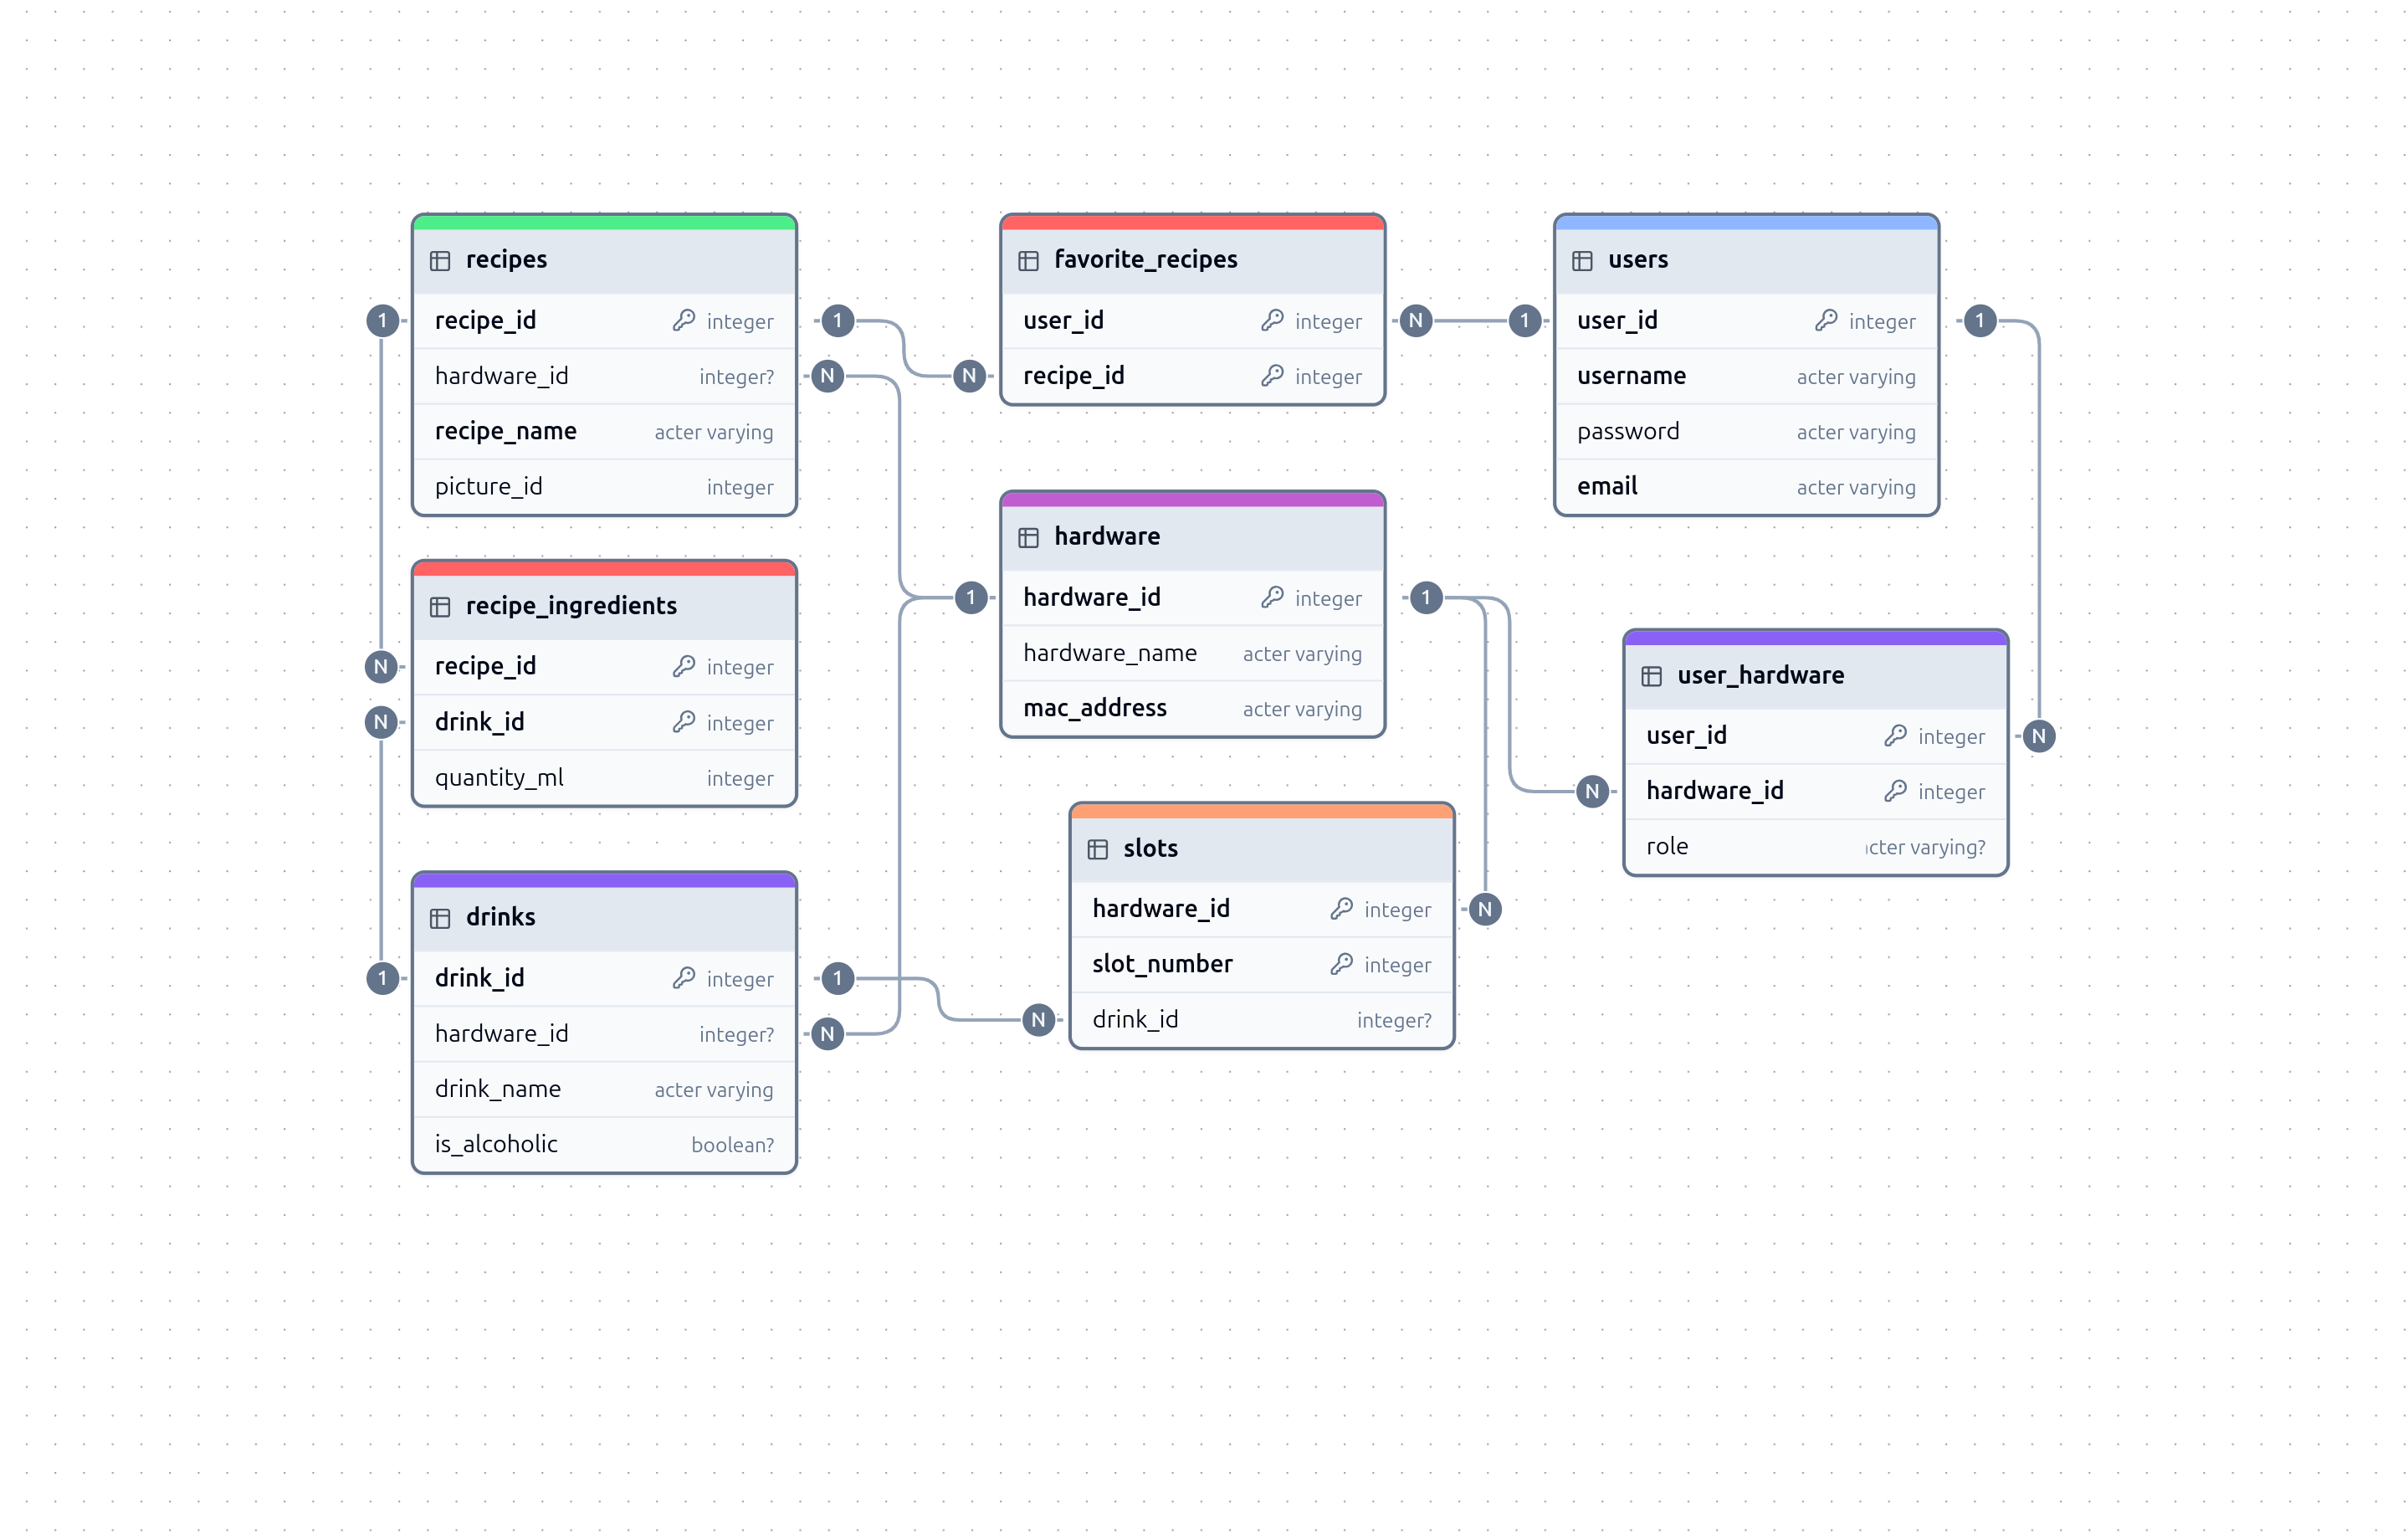
\includegraphics[height=0.9\textwidth, angle=90]{graphics/schemes/postgres_db_scheme.png}
  \caption{Datenbankdiagramm}
  \label{fig:database_diagram}
\end{figure}

\newpage

\subsection{Weiterer Anhang}    
\newpage

\section{Literaturverzeichnis}(1–2 Seiten)
% \section{Literaturverzeichnis}
% Hier folgt der Inhalt des Abschnitts "Literaturverzeichnis".

\printbibliography    
\newpage

\end{document}
